
%% bare_conf.tex
%% V1.3
%% 2007/01/11
%% by Michael Shell
%% See:
%% http://www.michaelshell.org/
%% for current contact information.
%%
%% This is a skeleton file demonstrating the use of IEEEtran.cls
%% (requires IEEEtran.cls version 1.7 or later) with an IEEE conference paper.
%%
%% Support sites:
%% http://www.michaelshell.org/tex/ieeetran/
%% http://www.ctan.org/tex-archive/macros/latex/contrib/IEEEtran/
%% and
%% http://www.ieee.org/

%%*************************************************************************
%% Legal Notice:
%% This code is offered as-is without any warranty either expressed or
%% implied; without even the implied warranty of MERCHANTABILITY or
%% FITNESS FOR A PARTICULAR PURPOSE!
%% User assumes all risk.
%% In no event shall IEEE or any contributor to this code be liable for
%% any damages or losses, including, but not limited to, incidental,
%% consequential, or any other damages, resulting from the use or misuse
%% of any information contained here.
%%
%% All comments are the opinions of their respective authors and are not
%% necessarily endorsed by the IEEE.
%%
%% This work is distributed under the LaTeX Project Public License (LPPL)
%% ( http://www.latex-project.org/ ) version 1.3, and may be freely used,
%% distributed and modified. A copy of the LPPL, version 1.3, is included
%% in the base LaTeX documentation of all distributions of LaTeX released
%% 2003/12/01 or later.
%% Retain all contribution notices and credits.
%% ** Modified files should be clearly indicated as such, including  **
%% ** renaming them and changing author support contact information. **
%%
%% File list of work: IEEEtran.cls, IEEEtran_HOWTO.pdf, bare_adv.tex,
%%                    bare_conf.tex, bare_jrnl.tex, bare_jrnl_compsoc.tex
%%*************************************************************************

% *** Authors should verify (and, if needed, correct) their LaTeX system  ***
% *** with the testflow diagnostic prior to trusting their LaTeX platform ***
% *** with production work. IEEE's font choices can trigger bugs that do  ***
% *** not appear when using other class files.                            ***
% The testflow support page is at:
% http://www.michaelshell.org/tex/testflow/



% Note that the a4paper option is mainly intended so that authors in
% countries using A4 can easily print to A4 and see how their papers will
% look in print - the typesetting of the document will not typically be
% affected with changes in paper size (but the bottom and side margins will).
% Use the testflow package mentioned above to verify correct handling of
% both paper sizes by the user's LaTeX system.
%
% Also note that the "draftcls" or "draftclsnofoot", not "draft", option
% should be used if it is desired that the figures are to be displayed in
% draft mode.
%
\documentclass[10pt, conference, compsocconf]{IEEEtran}
%\documentclass[conference]{IEEEtran}
% Add the compsocconf option for Computer Society conferences.
%
% If IEEEtran.cls has not been installed into the LaTeX system files,
% manually specify the path to it like:
% \documentclass[conference]{../sty/IEEEtran}


\usepackage{amsmath,amssymb,amsfonts} % 数学表达式
\usepackage{graphicx}  % 插入图片
\usepackage{float}
\usepackage{cite}
%\usepackage{subfigure}
\usepackage{subcaption}
\pagestyle{empty}% for cropping
\usepackage{amsthm}
\newtheorem{defn}{Definition}

\usepackage{algorithm,algcompatible,amsmath}
\DeclareMathOperator*{\argmax}{\arg\!\max}% https://tex.stackexchange.com/q/83169/5764
\algnewcommand\INPUT{\item[\textbf{Input:}]}%
\algnewcommand\OUTPUT{\item[\textbf{Output:}]}%
% Some very useful LaTeX packages include:
% (uncomment the ones you want to load)


% *** MISC UTILITY PACKAGES ***
%
%\usepackage{ifpdf}
% Heiko Oberdiek's ifpdf.sty is very useful if you need conditional
% compilation based on whether the output is pdf or dvi.
% usage:
% \ifpdf
%   % pdf code
% \else
%   % dvi code
% \fi
% The latest version of ifpdf.sty can be obtained from:
% http://www.ctan.org/tex-archive/macros/latex/contrib/oberdiek/
% Also, note that IEEEtran.cls V1.7 and later provides a builtin
% \ifCLASSINFOpdf conditional that works the same way.
% When switching from latex to pdflatex and vice-versa, the compiler may
% have to be run twice to clear warning/error messages.






% *** CITATION PACKAGES ***
%
%\usepackage{cite}
% cite.sty was written by Donald Arseneau
% V1.6 and later of IEEEtran pre-defines the format of the cite.sty package
% \cite{} output to follow that of IEEE. Loading the cite package will
% result in citation numbers being automatically sorted and properly
% "compressed/ranged". e.g., [1], [9], [2], [7], [5], [6] without using
% cite.sty will become [1], [2], [5]--[7], [9] using cite.sty. cite.sty's
% \cite will automatically add leading space, if needed. Use cite.sty's
% noadjust option (cite.sty V3.8 and later) if you want to turn this off.
% cite.sty is already installed on most LaTeX systems. Be sure and use
% version 4.0 (2003-05-27) and later if using hyperref.sty. cite.sty does
% not currently provide for hyperlinked citations.
% The latest version can be obtained at:
% http://www.ctan.org/tex-archive/macros/latex/contrib/cite/
% The documentation is contained in the cite.sty file itself.






% *** GRAPHICS RELATED PACKAGES ***
%
\ifCLASSINFOpdf
  % \usepackage[pdftex]{graphicx}
  % declare the path(s) where your graphic files are
  % \graphicspath{{../pdf/}{../jpeg/}}
  % and their extensions so you won't have to specify these with
  % every instance of \includegraphics
  % \DeclareGraphicsExtensions{.pdf,.jpeg,.png}
\else
  % or other class option (dvipsone, dvipdf, if not using dvips). graphicx
  % will default to the driver specified in the system graphics.cfg if no
  % driver is specified.
  % \usepackage[dvips]{graphicx}
  % declare the path(s) where your graphic files are
  % \graphicspath{{../eps/}}
  % and their extensions so you won't have to specify these with
  % every instance of \includegraphics
  % \DeclareGraphicsExtensions{.eps}
\fi
% graphicx was written by David Carlisle and Sebastian Rahtz. It is
% required if you want graphics, photos, etc. graphicx.sty is already
% installed on most LaTeX systems. The latest version and documentation can
% be obtained at:
% http://www.ctan.org/tex-archive/macros/latex/required/graphics/
% Another good source of documentation is "Using Imported Graphics in
% LaTeX2e" by Keith Reckdahl which can be found as epslatex.ps or
% epslatex.pdf at: http://www.ctan.org/tex-archive/info/
%
% latex, and pdflatex in dvi mode, support graphics in encapsulated
% postscript (.eps) format. pdflatex in pdf mode supports graphics
% in .pdf, .jpeg, .png and .mps (metapost) formats. Users should ensure
% that all non-photo figures use a vector format (.eps, .pdf, .mps) and
% not a bitmapped formats (.jpeg, .png). IEEE frowns on bitmapped formats
% which can result in "jaggedy"/blurry rendering of lines and letters as
% well as large increases in file sizes.
%
% You can find documentation about the pdfTeX application at:
% http://www.tug.org/applications/pdftex





% *** MATH PACKAGES ***
%
%\usepackage[cmex10]{amsmath}
% A popular package from the American Mathematical Society that provides
% many useful and powerful commands for dealing with mathematics. If using
% it, be sure to load this package with the cmex10 option to ensure that
% only type 1 fonts will utilized at all point sizes. Without this option,
% it is possible that some math symbols, particularly those within
% footnotes, will be rendered in bitmap form which will result in a
% document that can not be IEEE Xplore compliant!
%
% Also, note that the amsmath package sets \interdisplaylinepenalty to 10000
% thus preventing page breaks from occurring within multiline equations. Use:
%\interdisplaylinepenalty=2500
% after loading amsmath to restore such page breaks as IEEEtran.cls normally
% does. amsmath.sty is already installed on most LaTeX systems. The latest
% version and documentation can be obtained at:
% http://www.ctan.org/tex-archive/macros/latex/required/amslatex/math/





% *** SPECIALIZED LIST PACKAGES ***
%
%\usepackage{algorithmic}
% algorithmic.sty was written by Peter Williams and Rogerio Brito.
% This package provides an algorithmic environment fo describing algorithms.
% You can use the algorithmic environment in-text or within a figure
% environment to provide for a floating algorithm. Do NOT use the algorithm
% floating environment provided by algorithm.sty (by the same authors) or
% algorithm2e.sty (by Christophe Fiorio) as IEEE does not use dedicated
% algorithm float types and packages that provide these will not provide
% correct IEEE style captions. The latest version and documentation of
% algorithmic.sty can be obtained at:
% http://www.ctan.org/tex-archive/macros/latex/contrib/algorithms/
% There is also a support site at:
% http://algorithms.berlios.de/index.html
% Also of interest may be the (relatively newer and more customizable)
% algorithmicx.sty package by Szasz Janos:
% http://www.ctan.org/tex-archive/macros/latex/contrib/algorithmicx/




% *** ALIGNMENT PACKAGES ***
%
%\usepackage{array}
% Frank Mittelbach's and David Carlisle's array.sty patches and improves
% the standard LaTeX2e array and tabular environments to provide better
% appearance and additional user controls. As the default LaTeX2e table
% generation code is lacking to the point of almost being broken with
% respect to the quality of the end results, all users are strongly
% advised to use an enhanced (at the very least that provided by array.sty)
% set of table tools. array.sty is already installed on most systems. The
% latest version and documentation can be obtained at:
% http://www.ctan.org/tex-archive/macros/latex/required/tools/


%\usepackage{mdwmath}
%\usepackage{mdwtab}
% Also highly recommended is Mark Wooding's extremely powerful MDW tools,
% especially mdwmath.sty and mdwtab.sty which are used to format equations
% and tables, respectively. The MDWtools set is already installed on most
% LaTeX systems. The lastest version and documentation is available at:
% http://www.ctan.org/tex-archive/macros/latex/contrib/mdwtools/


% IEEEtran contains the IEEEeqnarray family of commands that can be used to
% generate multiline equations as well as matrices, tables, etc., of high
% quality.


%\usepackage{eqparbox}
% Also of notable interest is Scott Pakin's eqparbox package for creating
% (automatically sized) equal width boxes - aka "natural width parboxes".
% Available at:
% http://www.ctan.org/tex-archive/macros/latex/contrib/eqparbox/





% *** SUBFIGURE PACKAGES ***
%\usepackage[tight,footnotesize]{subfigure}
% subfigure.sty was written by Steven Douglas Cochran. This package makes it
% easy to put subfigures in your figures. e.g., "Figure 1a and 1b". For IEEE
% work, it is a good idea to load it with the tight package option to reduce
% the amount of white space around the subfigures. subfigure.sty is already
% installed on most LaTeX systems. The latest version and documentation can
% be obtained at:
% http://www.ctan.org/tex-archive/obsolete/macros/latex/contrib/subfigure/
% subfigure.sty has been superceeded by subfig.sty.



%\usepackage[caption=false]{caption}
%\usepackage[font=footnotesize]{subfig}
% subfig.sty, also written by Steven Douglas Cochran, is the modern
% replacement for subfigure.sty. However, subfig.sty requires and
% automatically loads Axel Sommerfeldt's caption.sty which will override
% IEEEtran.cls handling of captions and this will result in nonIEEE style
% figure/table captions. To prevent this problem, be sure and preload
% caption.sty with its "caption=false" package option. This is will preserve
% IEEEtran.cls handing of captions. Version 1.3 (2005/06/28) and later
% (recommended due to many improvements over 1.2) of subfig.sty supports
% the caption=false option directly:
%\usepackage[caption=false,font=footnotesize]{subfig}
%
% The latest version and documentation can be obtained at:
% http://www.ctan.org/tex-archive/macros/latex/contrib/subfig/
% The latest version and documentation of caption.sty can be obtained at:
% http://www.ctan.org/tex-archive/macros/latex/contrib/caption/




% *** FLOAT PACKAGES ***
%
%\usepackage{fixltx2e}
% fixltx2e, the successor to the earlier fix2col.sty, was written by
% Frank Mittelbach and David Carlisle. This package corrects a few problems
% in the LaTeX2e kernel, the most notable of which is that in current
% LaTeX2e releases, the ordering of single and double column floats is not
% guaranteed to be preserved. Thus, an unpatched LaTeX2e can allow a
% single column figure to be placed prior to an earlier double column
% figure. The latest version and documentation can be found at:
% http://www.ctan.org/tex-archive/macros/latex/base/



%\usepackage{stfloats}
% stfloats.sty was written by Sigitas Tolusis. This package gives LaTeX2e
% the ability to do double column floats at the bottom of the page as well
% as the top. (e.g., "\begin{figure*}[!b]" is not normally possible in
% LaTeX2e). It also provides a command:
%\fnbelowfloat
% to enable the placement of footnotes below bottom floats (the standard
% LaTeX2e kernel puts them above bottom floats). This is an invasive package
% which rewrites many portions of the LaTeX2e float routines. It may not work
% with other packages that modify the LaTeX2e float routines. The latest
% version and documentation can be obtained at:
% http://www.ctan.org/tex-archive/macros/latex/contrib/sttools/
% Documentation is contained in the stfloats.sty comments as well as in the
% presfull.pdf file. Do not use the stfloats baselinefloat ability as IEEE
% does not allow \baselineskip to stretch. Authors submitting work to the
% IEEE should note that IEEE rarely uses double column equations and
% that authors should try to avoid such use. Do not be tempted to use the
% cuted.sty or midfloat.sty packages (also by Sigitas Tolusis) as IEEE does
% not format its papers in such ways.





% *** PDF, URL AND HYPERLINK PACKAGES ***
%
%\usepackage{url}
% url.sty was written by Donald Arseneau. It provides better support for
% handling and breaking URLs. url.sty is already installed on most LaTeX
% systems. The latest version can be obtained at:
% http://www.ctan.org/tex-archive/macros/latex/contrib/misc/
% Read the url.sty source comments for usage information. Basically,
% \url{my_url_here}.





% *** Do not adjust lengths that control margins, column widths, etc. ***
% *** Do not use packages that alter fonts (such as pslatex).         ***
% There should be no need to do such things with IEEEtran.cls V1.6 and later.
% (Unless specifically asked to do so by the journal or conference you plan
% to submit to, of course. )


% correct bad hyphenation here
\hyphenation{op-tical net-works semi-conduc-tor}


\begin{document}
%
% paper title
% can use linebreaks \\ within to get better formatting as desired
%-------------------------------------------------------------------------------标题
% 换行//
\title{MBDI: A General Paradigm for Mixed Loop Boundary Dynamic issues On CGRAs}

% author names and affiliations
% use a multiple column layout for up to two different
% affiliations

%\author{\IEEEauthorblockN{Shuai Xie, Zhongyuan Zhao, Weiguang Sheng, Qin Wang}
%\IEEEauthorblockA{Department of Micro/NaNo Electronics, Shanghai Jiao Tong University\\
%%line 2: name of organization, acronyms acceptable\\
%Shanghai, China\\
%Email: xiaoxiyouran@sjtu.edu.cn}
%%\and
%%\IEEEauthorblockN{Authors Name/s per 2nd Affiliation (Author)}
%%\IEEEauthorblockA{line 1 (of Affiliation): dept. name of organization\\
%%line 2: name of organization, acronyms acceptable\\
%%line 3: City, Country\\
%%line 4: Email: name@xyz.com}
%}

% conference papers do not typically use \thanks and this command
% is locked out in conference mode. If really needed, such as for
% the acknowledgment of grants, issue a \IEEEoverridecommandlockouts
% after \documentclass

% for over three affiliations, or if they all won't fit within the width
% of the page, use this alternative format:
%
%\author{\IEEEauthorblockN{Michael Shell\IEEEauthorrefmark{1},
%Homer Simpson\IEEEauthorrefmark{2},
%James Kirk\IEEEauthorrefmark{3},
%Montgomery Scott\IEEEauthorrefmark{3} and
%Eldon Tyrell\IEEEauthorrefmark{4}}
%\IEEEauthorblockA{\IEEEauthorrefmark{1}School of Electrical and Computer Engineering\\
%Georgia Institute of Technology,
%Atlanta, Georgia 30332--0250\\ Email: see http://www.michaelshell.org/contact.html}
%\IEEEauthorblockA{\IEEEauthorrefmark{2}Twentieth Century Fox, Springfield, USA\\
%Email: homer@thesimpsons.com}
%\IEEEauthorblockA{\IEEEauthorrefmark{3}Starfleet Academy, San Francisco, California 96678-2391\\
%Telephone: (800) 555--1212, Fax: (888) 555--1212}
%\IEEEauthorblockA{\IEEEauthorrefmark{4}Tyrell Inc., 123 Replicant Street, Los Angeles, California 90210--4321}}




% use for special paper notices
%\IEEEspecialpapernotice{(Invited Paper)}




% make the title area
\maketitle

%-------------------------------------------------------------------------------Abstract
\begin{abstract}
%The abstract goes here. DO NOT USE SPECIAL CHARACTERS, SYMBOLS, OR MATH IN YOUR TITLE OR ABSTRACT.
Coarse Grained Reconfigurable Architectures (CGRAs) have been recognized as desirable platform for repetitive, datapath-oriented and computational intensive applications. One of the primary challenges is to develop compilers that can produce high efficient commands for CGRAs. An important aspect of compiler is the optimization for irregular applications. To this end, this paper makes several contributions: i) Treating loop itself as operations to dynamically control the execution of innermost loop body, which is described as $DBDI$. For the first time in CGRA compilers, we proposed the use of loop operations as a general solution for different kinds of loops. ii) A rule is presented for irregular applications to dispose loop itself and innermost loop body creatively. The arrangement of control flow and placement for loop is amenable.  iii) Mixed boundary and dynamic issues(MBDI) method is also introduced to improve the efficiency. MBDI employs the skillful approach that static boundary statically compile,dynamic boundary dynamically execute to reduce both operations and power dramatically.An evaluation is drafted finally under this framework which is accessible to process the data flow with its high quality as well as handcraft. As a result, up to 4x speed up greater than a conventional high-level compile tools. MBDI is capable of achieving the theoretical best performance based on any benchmarks as we practiced. As long as the operation number of loop body is greater than 2, the performance ratio and power ratio remain invincible.
\end{abstract}

\begin{IEEEkeywords}
Coarse Grained Reconfigurable Architectures; processing element arrays; DBDI; MBDI;

\end{IEEEkeywords}


% For peer review papers, you can put extra information on the cover
% page as needed:
% \ifCLASSOPTIONpeerreview
% \begin{center} \bfseries EDICS Category: 3-BBND \end{center}
% \fi
%
% For peerreview papers, this IEEEtran command inserts a page break and
% creates the second title. It will be ignored for other modes.
\IEEEpeerreviewmaketitle


%-------------------------------------------------------------------------------Introduction
\section{Introduction}
% no \IEEEPARstart
%Nowadays, the improvement of concurrency on instruction and data promotes the development of $spatially-programmed$ such as field-programmable gate arrays(FPGAs) and CGRAs. 
To achieve the targets of high power efficiency, most of research on data flow mapping\cite{bg-epimap}, aggressive pipeline\cite{bg-aggressive} and triggered instructions\cite{bg-triggered} have been exploited in recent years. CGRA occupies the spatial parallelism structure to accelerate classic workload genres. However, it's not adequate to facilitate a few irregular applications with uncertain boundary loop or forcible data/control dependency. Therefore, the performance on speed and energy is limited by compiler, especially for nonuniform programs, even though an efficient hardware is available\cite{bg-operation}.

During the past decade, much pioneer work has been focused on flattening-based mapping of imperfect loop nests\cite{in-flattening}, non-kernel execution times\cite{in-kim2012improving}, graph minor\cite{in-chen2014graph}, polyhedral model on mapping\cite{in-liu2013polyhedral}, sub-cycle modulo scheduler\cite{in-park2009cgra} and so on. A majority of compilers cater to the process of data flow graph(DFG) mapping and reduction of initiation interval($II$) by simplifying programs delicately. Nevertheless, there is still no thorough schemes for all applications. Just as approaches for the optimization of uncertain loop boundary are desired eagerly for a number of applications since it's a margin territory but unavoidable.

In this paper, we take the first step on putting forward dynamic boundary, dynamic issue($DBDI$), an innovative method for data pipelining of loops on processing element(PE) arrays aims at highly simultaneous. What’s more, to lessen operations and economize power, mixed boundary, dynamic issue(MBDI), as another creative technique is feasible to extract more computational throughout. Though it is available to high efficiency and significant performance on speed or power consumption for CGRA, whether can be implemented is critically limited by the compiler technologies.
There are three questions must be figured out before an application is allocated to processing element arrays(PEA): i) how to arrange the flow of instructions on loop pipelining to decrease initiation interval($II$). ii) where are the operations placed. iii) what is the communication among PEs through router.
Actually, these three problems can be summarized to : scheduling, placement and routing.
On account of these difficulties, predicted execution\cite{mo-wang2015acceleration} has proposed an efficent way for $if$ branch. But this paper presents an opportunity for $loop$.
%``search base''\cite{in-clark2005architecture}, EPIMap\cite{bg-epimap} and SPDI\cite{in-zhao2017static} have been published to find out state-of-the-art technology for applications mapped to CGRA.


Owing to the restrictions of previous work based on static loop boundary, much inevitable trouble may be encountered when nonuniform loops with dynamic boundary occurs. Three breakthroughs on CGRA are presented in this paper:\\
\textbf{1. Realization of dynamic loop, dynamically execute:} The benefits of array topology is to expedite the calculation, particularly the $SIMD$. Whereas, it is a great challenge to accommodate the dynamic boundary loop.
In general, pipelining is utilized to parallelize programs, and at a fixed interval, implementing the same operations. To fit the architecture, $DBDI$ takes an important role in scheduling instructions subtly.\\
\textbf{2. Establishing a rule for loop mapping:} Previously, plenty of CGRA structure have been raised, including HSRA\cite{in-tsu1999hsra}, MATRIX\cite{in-mirsky1996matrix}, RaPiD\cite{in-hartenstein1996field}, Tartan\cite{in-mishra2007virtualization}, MorphoSys\cite{in-singh2000morphosys}. Each of the projects mentioned above requires custom mapping tools that supports a limited subset of structure features\cite{in-friedman2009spr}. In order to fulfill the gap in previous mapping techniques, we set up a rule to process extra loop instructions. The control flow is also described simultaneously. \\
\textbf{3. Extracting an universal principle for mixed loop boundaries:} Traditional loops are compiled statically to operate the innermost loop body, extra overhead will be occupied if all loop operations cover the same patterns. It employs much more energy for the static instructions, but only dynamic boundary judgment is demanded. In this case, static compiling the static loop boundary and dynamic committing the task of dynamic loop orient to any applications moderately. Furthermore, sophisticated mapping of control flow is crucial to the pipelining.

Consequently, we evaluate the $DBDI$ model, and an improved methodology($MBDI$) by simulating several classic kernels as workload. According to 15 benchmarks\cite{ev-asanovic2006landscape,ev-henning2006spec}, experiments reveal that the performance on irregular programs is dramatically more efficient than those high-level compile tools as we known currently. Our approach can generate almost 2x average performance ratio compared to traditional solutions of static boundary, static issues($SBSI$).

%-------------------------------------------------------------------------------Background and motivation
\section{Background and Motivation}
PEA is used as the computation vector, composed of 4$\times$4 array(16PEs) and internal connection. Otherwise, a shared memory is provided for data storage. Each PE includes an arithmetic logical unit(ALU), a local register file and a output register, which retains the data for local PE or neighboring PE at next clock. As Fig. \ref{fig_pearray} depicted, there are two coarse input($IN1$, $IN2$) for computation. It is important to note that input $IN3$ is applied in the control flow, ALU is enable if $IN3 = 0$, otherwise, ALU is idle. Although $IN3$ may be not emerged in most literature, it is necessary to control running in reality. What's more, inter-PEs transfer data through router.

%PEA is adapted as coarse grained accelerator, most of work is to study the improvement of flexibility and efficiency. For example, trigger instruction set \cite{bg-triggered}, eliminating the program counter and avoid over-serialize execution. Moreover, many schemes have been taken on the acceleration of control flows for branch instructions \cite{mo-wang2015acceleration}. Last but not least, aggressive pipeline \cite{bg-aggressive} put forward a blueprint of eliminating data dependency and optimizing datapath.

PEA is adopted as coarse grained accelerator, most of work is to study the improvement of flexibility and efficiency. For example, partial predication and full predication\cite{mo-parashar2014efficient} or even composite predication\cite{mo-wang2015acceleration}. Most of work is focused on $if-else$ structure. But what about loop $for$, or even $for-if$ or $while-if$?

So far much study has exploited on $if-else$  and innermost loop body\cite{in-kim2012improving}. Besides, new parallelism framework is provided for instruction execution and solving the data dependency of innermost loop body by an explicit datapath. However, it's important to note that a headache problem for the acceleration of control flows with loop instruction still remains. It is a new topic for irregular loop applications and worthwhile for us to emerge an efficient approach but not only feasible.

Many irregular control flows for loop in Fig. \ref{fig_tab} are displayed. In summary, there are three kinds of irregular loops to be solved: i) It is really difficult for us to arrange the operation of loop mixed because most applications are only focused on regular statements. Such as $for-if$ mixed in bucket sort, $while-if$ mixed in Fibonacci Search, execution operations mixed in autocr. ii) Loop itself is treated as operations. Such an instruction is often adopted to the kind of sort algorithm, for example in Binary Search. iii) Loop is not certain ahead of run-time. As we listed, the initialization value of loop is uncertain in SPMV and LU, loop boundary is mutable in DFS, loop step is float in Knapsack Problem. Since only static loop operations are considered for most high-level synthesis tools. In other words, if there is a blurry instruction block, this application may be not appropriate for CGRA, application scenarios to a great extent is limited. To unite statement, it will be named as dynamic loop in this paper if the loop boundary is uncertain. Otherwise, static loop is accessible for fixed boundary.
\begin{figure}[!t]
	\centering
	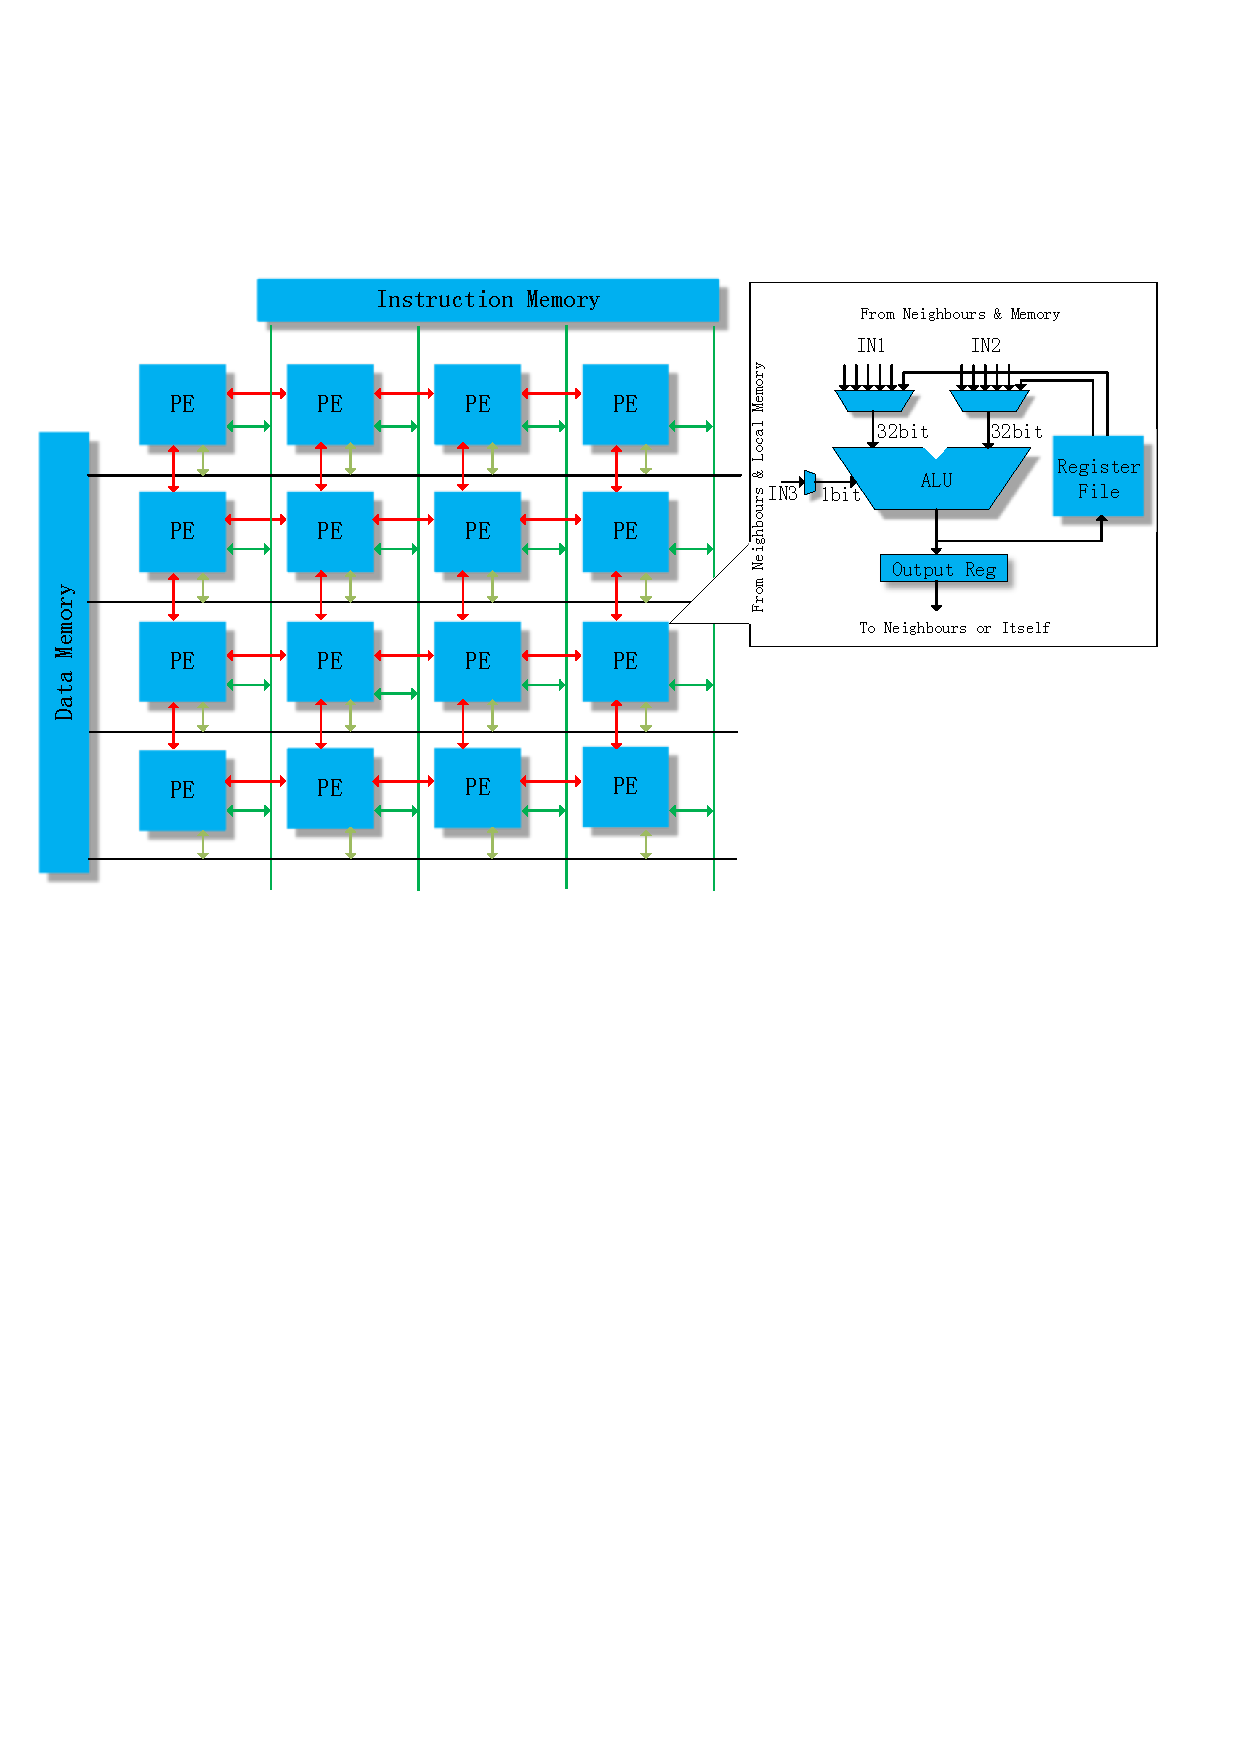
\includegraphics[width=0.45\textwidth]{fi/Pe_arrays.pdf}
	\caption{The structure of 4x4 PEs inside CGRA computing model, composed of ALU, output register, local register file.}
	\label{fig_pearray}
\end{figure}
%
%For bucket sort,
%
%When the loop boundary is uncertain, the execution of DFS algorithm present a great challenge for compiler.
%
%In another case, For example, $while$ or $for$ statement is viable to find out the index of an array in Binary Search kernel. In traditional framework, this kind of operation may be translated to branch instruction, although a complicated control flow is required or even no valid approach to recongnize when the application get out of the function and when it continue running.
%
%It will be unacceptable for the case that general programs mixed with uncertian loops according to Auctor, which is described as imperfect loops.
%In Fibonacci Search kernel, hybrid instructions for $while$ and $if$ in one block are divided into two parts in previous compile tools. Meanwhile, there is a huge challenge on how to compile it together.
%
%The status of different initialization value in $for$ sentence is also common in applications, which can be verified in SPMV kernel.
%
%Moreover, the step of each loop is likely to be changed as we see in Knapsack Problem.
%
%In addition, it might be worse if $for$ sentence depends on previous $while$ as shown in LU kernel.
%

All in all, so many irregular applications are hard to manage, but they are general in classic algorithms. Hence a novel scheme is valuable to address the full opportunities. Although we prefer to present the problem iii) in the paper, other situations are amenable to be processed in the same methodology. Details on the previous methods are discussed in next section, then a high efficient one is carried out later.
\begin{figure*}[!t]
	\centering
	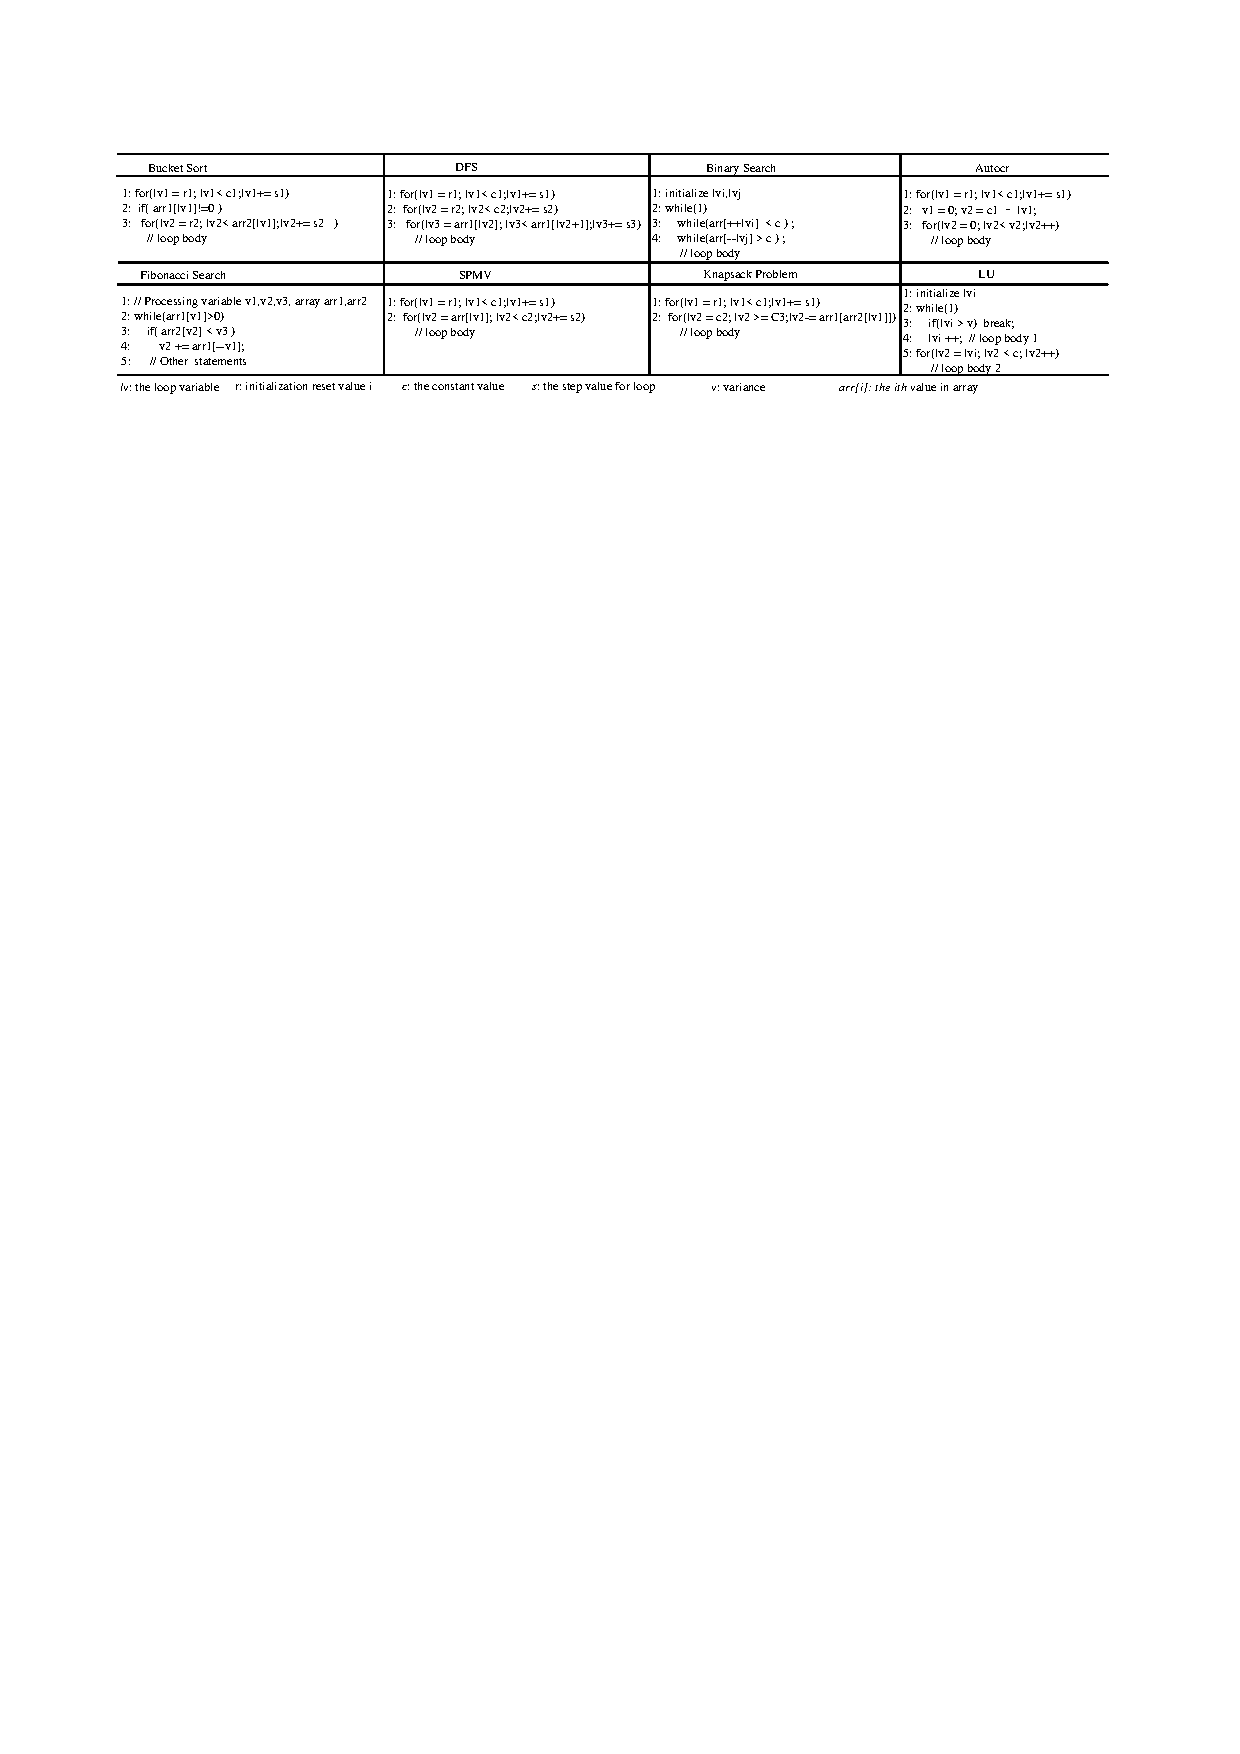
\includegraphics[width=0.9\textwidth]{fi/tab.pdf}
	\caption{Kinds of loop function in benchmarks.}
	\label{fig_tab}
\end{figure*}
% You must have at least 2 lines in the paragraph with the drop letter
% (should never be an issue)
%-------------------------------------------------------------------------------Background and motivation
\section{Related Work}
As we mentioned earlier in section 1, three prominent questions must be overcomed in compiler. Furthermore, it is related to map, scheduling and routing in loop data flow graph (DFG). It is recognized that  the synthesis tools have significant influence on the performance for general applications. Most research has focused on how to mapping and schedule for innermost loop body, including branch instructions \cite{re-ahn2006spatial,re-dimitroulakos2006exploring,re-friedman2009spr,re-guo2006pattern,re-hatanaka2007modulo,re-lee2003compilation}. Whereas, the irregular applications are not rare for general kernel, especially in search and sort domains. This paper takes the first step to discuss these questions, a traditional approach we named as static boundary, static issue(SBSI), which is used to make a contrast. In terms of simple dynamic boundary in a loop, the maximum loop times is adopted to the whole loop boundary. It is helpful for us to find the best schemes currently even though it is not familiar for us to study the best program in this new area so far. Perhaps based on one of the feasible methods, we will present a novel method closed to ideal situation by handcraft. 

%,re-mei2004design
As far as we concerned, SBSI is an optional approach to dispose uncertain boundary loop. However, several drawbacks are clear for SBSI. It is feasible  that only the kind of application whose boundary are available for us to obtain in compile time not in run-time. At the same time, many invalid iteration are also executed with branch instructions to guarantee its accuracy, which are not efficient because much more run time and power are required. As a result, irregular loop applications contradict with the demand of high efficiency and low power in CGRA.

Proper hardware and software combination allow us to systematically solve the irregular loop applications. Then, the concept of $DBDI$ are explained firstly, and the accuracy are important to be verified too. What’s more, more valid strategies are presented to promote $II$ and eliminate operations as possible as we can. Finally, an unified algorithm is achieved naturally before we show the experimental results.

%-------------------------------------------------------------------------------Background and motivation
\section{DBDI}
In this section, the general uncertain loop structure is simplified in terms of DFG to decrease the $II$. In addition, details on the aspect of $DBDI$ is represented exactly step by step. Furthermore, the bottleneck of $DBDI$ on the $II$ is reduced to 2, or even 1.
\begin{figure*}[!t]
	\centering
	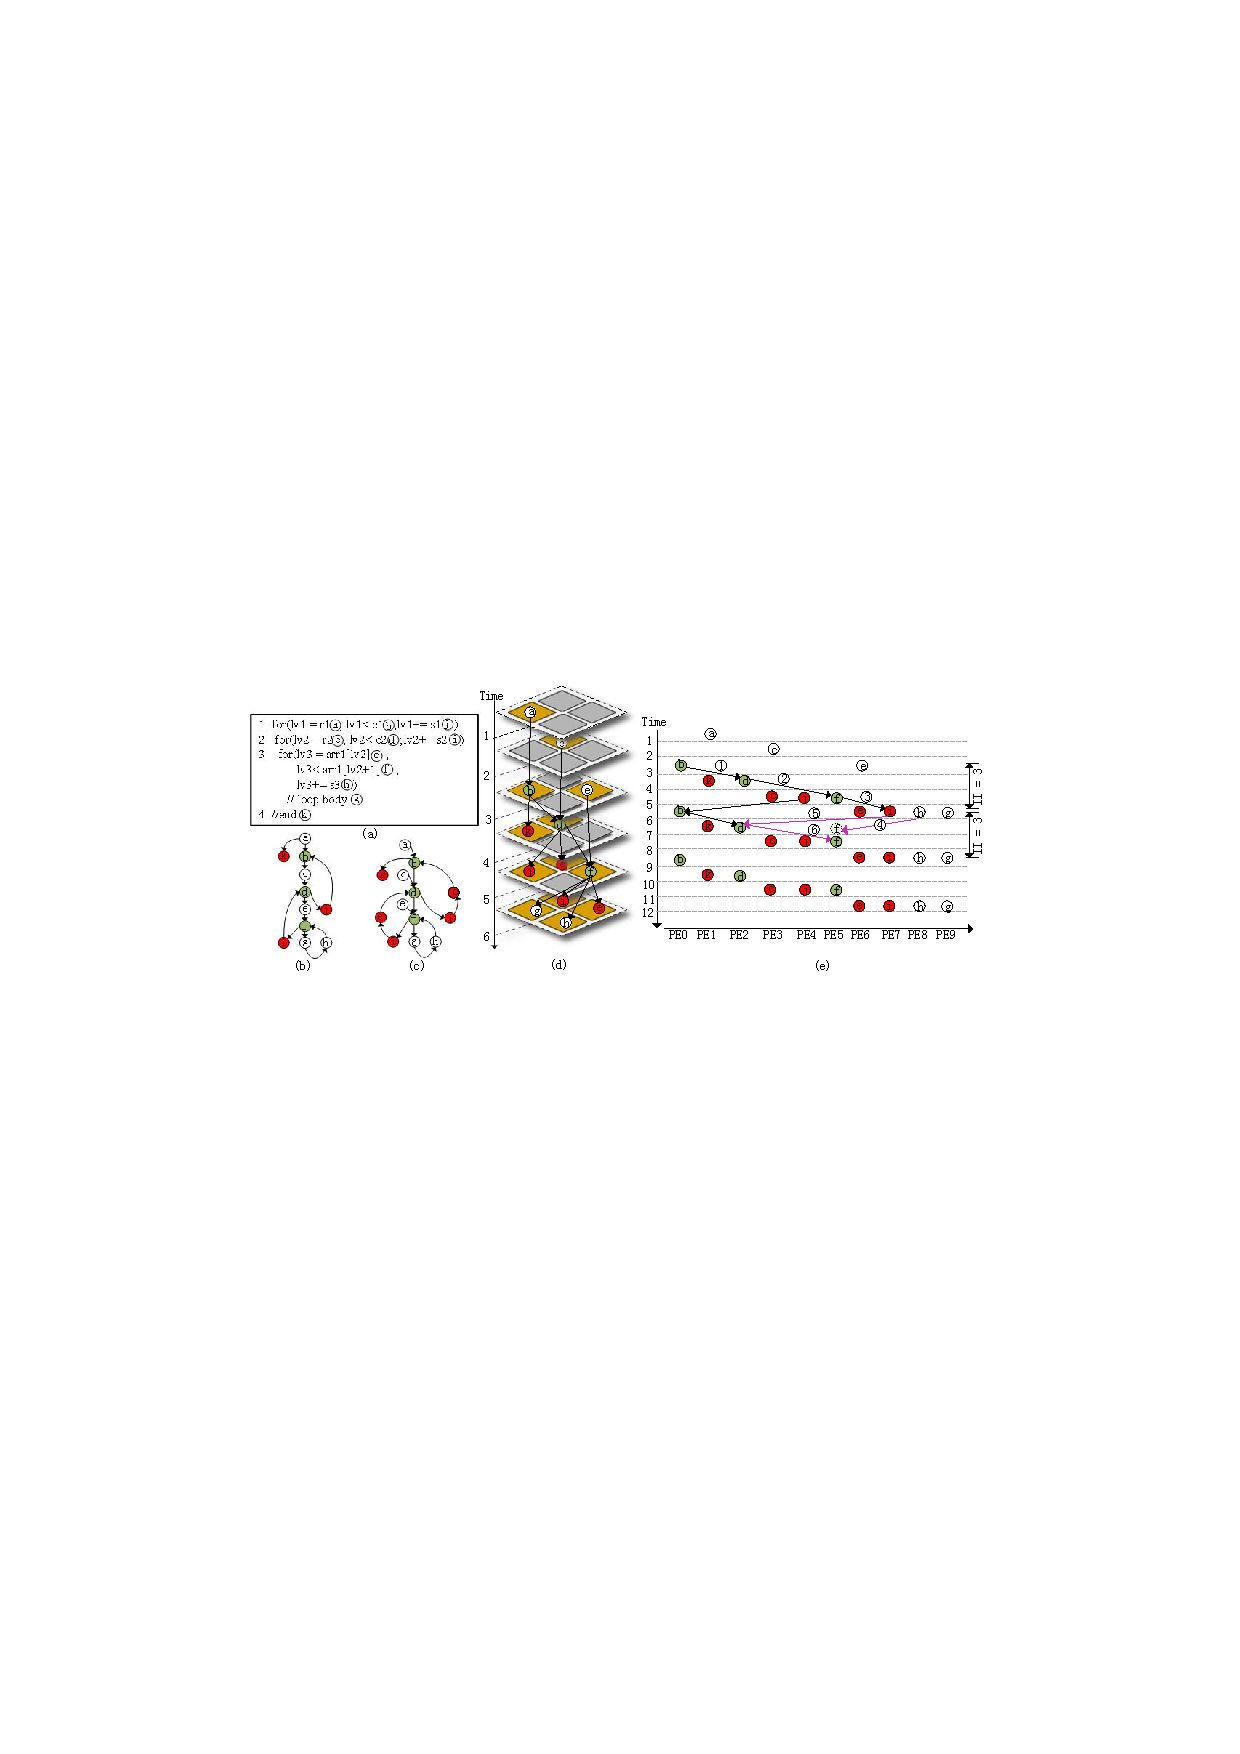
\includegraphics[width=0.9\textwidth]{fi/dfg.pdf}
	\caption{(a) Loop program flow of DFS, (b) DFG of loop, (c) simplified DFG, (d) scheduling of the instructions on the 2$\times$2 PEs, which is time extended, (e) mapping of three-layer loops, the minimum $II$ is 3.}
	\label{fig_dfg}
\end{figure*}
\subsection{Overview}
DFS kernel is chosen to describe the problem due to its classic and characteristic with three-level loop. As shown in Fig. \ref{fig_dfg}(a), indentation indicates a program block and each operation is tagged from $a \sim k$. we simplify inner loop body as only one line issue $g$ to focus insight on the feasibility and accuracy of $DBDI$ owing to the mature technique of mapping, scheduling, and placing for innermost loop body already \cite{re-guo2006pattern, re-hatanaka2007modulo, re-park2008edge, re-ahn2006spatial, re-friedman2009spr, re-yoon2009graph, bg-operation, in-flattening,in-chen2014graph, in-liu2013polyhedral, in-friedman2009spr}. The loop boundary of the two outermost levels is static, then compiler runs a such application with fixed step, times and reset value. Above all, it is the characteristic of SBSI.

In the following sections, data flow graph(DFG) and an improved-DFG are introduced. We take the first step of the mapping and scheduling for the applications with dynamic loop boundary.
\subsection{ Improved-DFG}
Fig. \ref{fig_dfg}(b) drafts the DFG, which is a directed graph $D = (V_d,E_d)$ where nodes represent for issue and $Ed$ stands for the link between nodes, and arc $(a,b)\in E_d$ iff the output of operation $a$ is an input of operation $b$ \cite{bg-epimap}. The directed graph expresses that $b$ is executed after $a$ completed, which indicates the time scale of nodes. According to the order of execution in Fig. \ref{fig_dfg}(a), program begins at $a$, then judges at $b$, line 2 is accessible if the judgment is true, or line 4 is on the line. Lastly, the loop variable $j$ is updated.

Improved-DFG is displayed ahead in Fig. \ref{fig_dfg}(c), given graph $D=(V_d,E_d)$, let $n$ be the number of nodes in $Vd$, that is, $n = \left|V_d\right|$. A node is described by $n_i = (v_i,e_i)\in D, e_i=(i,r), 1\leq \forall i \leq n$, let $C =(V_c,E_c)$ be the time extended CGRA(TEC)\cite{bg-epimap}, let $C_i$ be a subset of $C$, ie, $C_i \subseteq C$. Define $S=\{S_1,S_2,\cdots,S_n\}$ is the set of sub graph, $S_i$ is consist of adjacent nodes. Then, we give the definition of \textbf{critical path},

\begin{defn} Assuming that there is a node $n_z=(v_{z},e_{z})\in D,e_{z} = (z,r)$, $1 \leq \forall z,\forall r \leq n$ at least has two pre nodes that satisfy $\exists n_p = (v_{p},e_{p}) \in D, e_{p}=(p,z), 1 \leq \forall p \leq n$, and $\exists n_q = (v_{q},e_{q}) \in D, e_{q}=(q,z), 1 \leq \forall q \leq n$. Then $\exists S_{pz}, \{n_p,n_z\} \subseteq S_{pz}, \exists C_{pz}, C_{pz}\subseteq C, 1 \leq \forall pz \leq n$, at the same time, $\exists S_{qz}, \{n_q,n_z\}\subseteq S_{qz}, \exists C_{qz}, C_{qz} \subseteq C, 1 \leq \forall qz \leq n$, the longest path $max\{C_{pz},C_{qz}\}$ is the \textbf{critical path}. \end{defn}

In Fig. \ref{fig_dfg}(b), the red circle is selected if the judgment(green circle) is false. From \textit{Definition 1}, the green circle is the node($n_z$) that we look for. There are at least two nodes referred to it, thus two datapaths are achievable. As for PEA, it operates in the form of pipelining, the interval of the next loop is noted as $II$ generally. And designers always try every effort to cut down it. With regards to node $n_z$, we choose the critical path to decide $II$. Accordingly, a $C$ is available to TEC.

As above analyzed, we long to reduce the length of critical path to reduce $II$. Because no other operations except $for/while$ between line 1 and line 3 in Fig. \ref{fig_dfg}(a). So the reset nodes($a$,$c$,$e$) can move to another path in  Fig. \ref{fig_dfg}(c). It is beneficial to compress $II$, thanks to tuned nodes($a$,$c$,$e$) owning concurrency after the startup of loop. It is clearly shown in  Fig. \ref{fig_dfg}(d), $c$ is excuted with $f$ at time 5, and $e$ is available with $g,h$. It is easy to verify that the functionality remains when DFG is converted into Fig. \ref{fig_dfg}(c).

\subsection{Dynamic Boundary Dynamic Issue}
As shown explicitly in Fig. \ref{fig_dfg}(d), because the space is limited, we employ 2$\times$2 PEA to present TEC, which displays the scheduling of DFG. And the grey blocks may be utilized for another issues in a new iteration. In Fig. \ref{fig_dfg}(d), node $d$ is executed at $t = 4$. Two paths are accessible($a\--b\--d $ and $c\--d$), it is clear that $a\--b\--d $ is the critical path. In Fig. \ref{fig_dfg}(e), operations are unfolded explicitly. 

To illustrate the time scale and mapping of DFG elaborately, we allocate each issue in a single PE as disposed in Fig. \ref{fig_dfg}(e). The placement of nodes is determined by its dependency. Arrows in figure represents different paths. For example, two purple arrow lines reveal the feasible execution paths of node $f$. The earliest time of operation for path 4 is $t=7$, but path 6 is $t=8$. Therefore, path 6 represents for the critical path.

Above all, the minimal $II$ is 3 through improved-DFG. However, it is not the best one if the number of operations in innermost loop body is smaller than 3. Next section will address this problem directly.

%\hfill mds
%
%\hfill August 26, 2015

\subsection{Improved-DBDI}
Apart from scheduling, placing and routing of data transfer on PE, the controlling is also on the agenda. Each PE owns a control fine port($IN3$) which is responsible for the activation of ALU. Thus, not only routing for data transaction is in need, but also routing for control is significant. We consider a \textbf{rule} for the arrangement of control flow and data dependency in the loops:
\begin{defn}A \textbf{rule} is a promise to control the execution of issues from outside to inside, but $II$ of TEC is transferred from inside to outside.
\end{defn}
\begin{figure*}[!t]
	\centering
	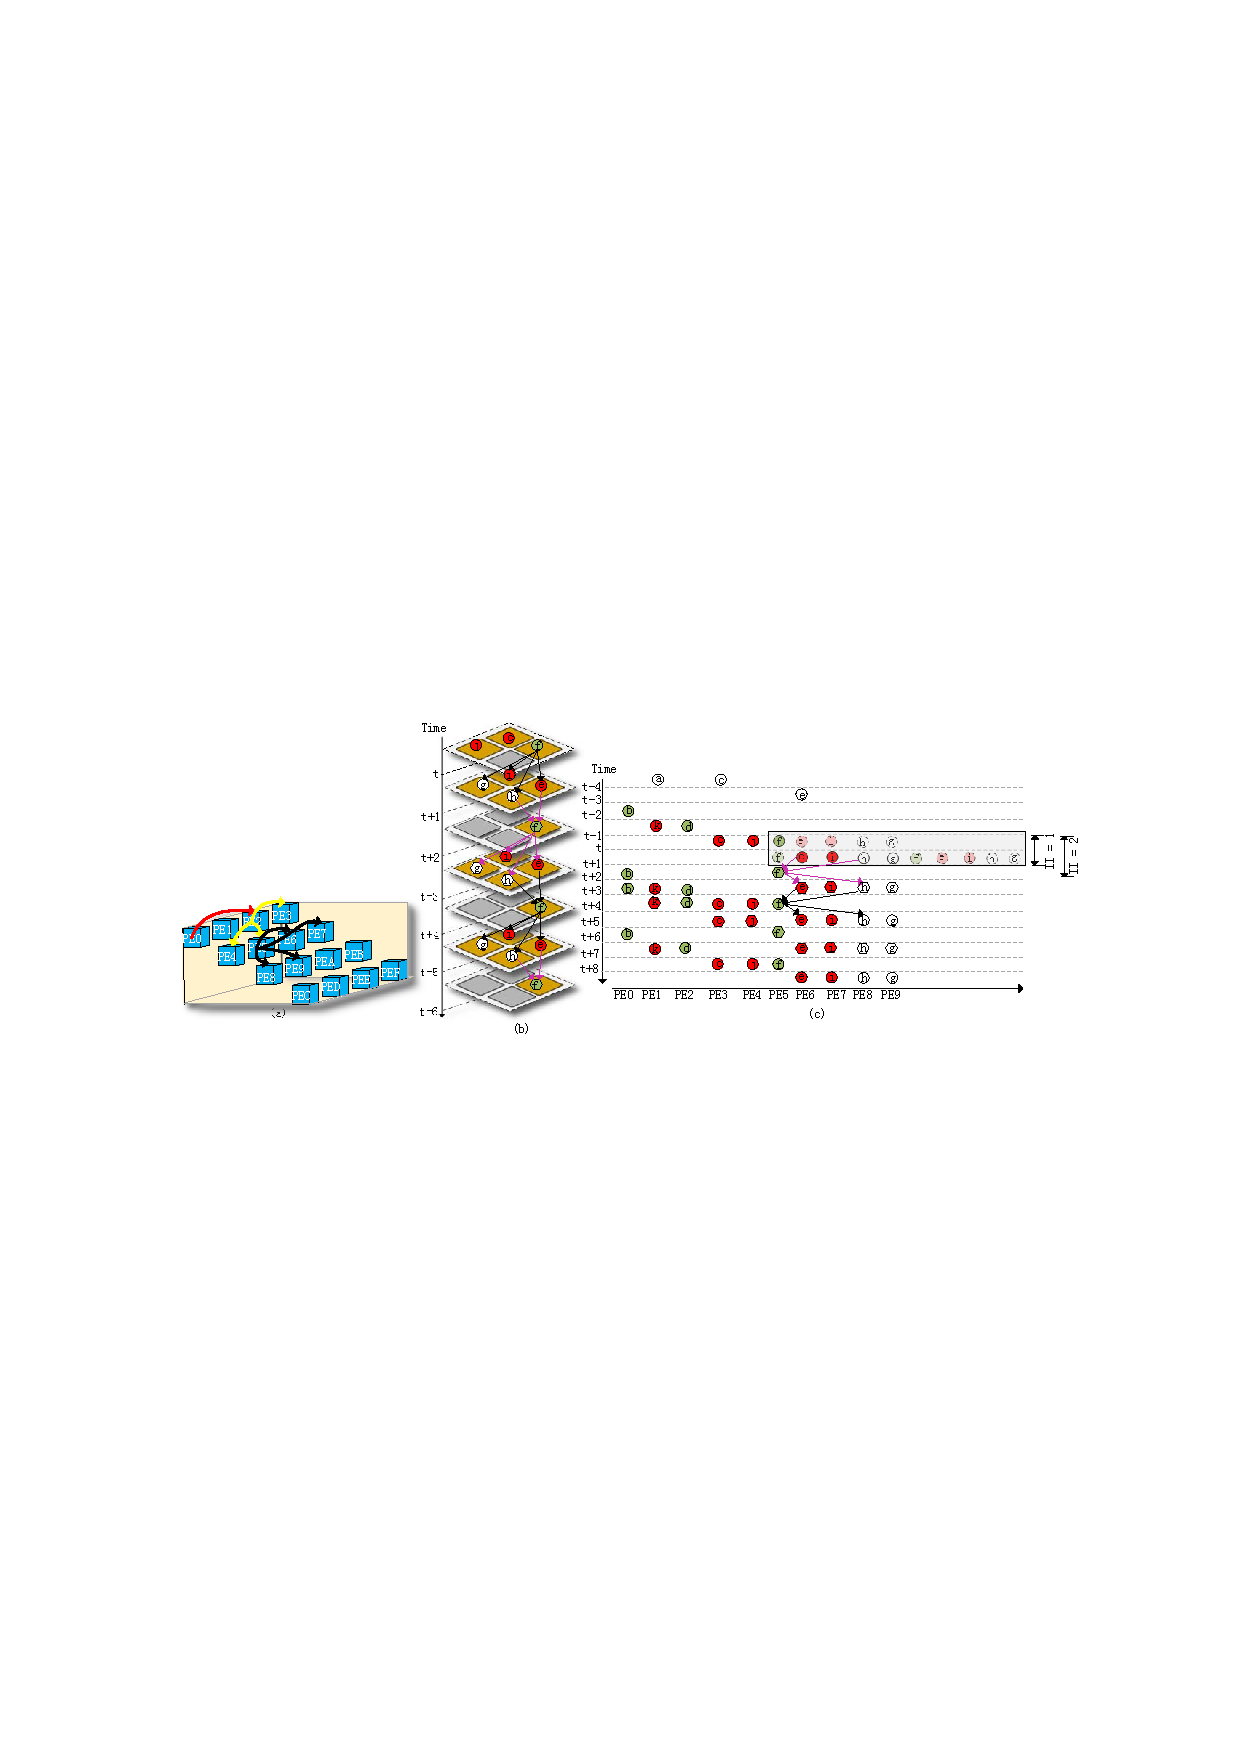
\includegraphics[width=0.9\textwidth]{fi/pe_cfg.pdf}
	\caption{(a) The dependency of control flow among PEs, thus input $IN3$ of PE2 is from PE0. In the same way, $IN3$ of PE3/4/5 is from PE2, (b) on 2$\times$2 PEA, cross execution of inner loop, which is tiled on TEC, (c) mapping and time scale of three-layer loops, the $II$ of cross execution is 2, the minimal value is 1 extremely.}
	\label{fig_pe_cfg}
\end{figure*}
Considering the judgment of outer loop node $n_{z\_o}=(v_{z\_o}$, $e_{z\_o}) \in D$, $e_{z\_o}=(z\_o,z\_ro)$, $1 \leq \forall z\_o, \forall z\_ro \leq n$ and the judgment of inner loop node $n_{z\_i}=(v_{z\_i},e_{z\_i}) \in D,e_{z\_i}=(z\_i,z\_ri), 1 \leq \forall z\_i, \forall z\_{ri} \leq n$,  there is an adjacent link between $n_{z\_o}$ and $n_{z\_i}$, where an arc $e_{z\_o}=(z\_o,z\_ro)$ is the bridge of $n_{z\_o}$ and $n_{z\_i}$. As we expected, loop is initialize form outside to inside, direction of the arc is pointed to inner loop nodes. Therefore, the control flow starts at outer loop, which caters to the operation pattern of pipelining. Communication for control is associated with Fig. \ref{fig_pe_cfg}(a).

In fact the dependency among loop variables, such as $lv1$,$lv2$,$lv3$ in Fig. \ref{fig_dfg}(a), is likely to be deemed as stack. The stack is established $S_t=\{S_{lv1},S_{lv2},S_{lv3}\}$, while judgment nodes $n_{z\_lv1},n_{z\_lv2},n_{z\_lv3}\in S_{lv1}$; $n_{z\_lv2},n_{z\_lv3}\in S_{lv2}$; $n_{z\_lv3}\in S_{lv3}$, besides $S_{lv1},S_{lv2},S_{lv3}\subseteq S$.
The order of running is elucidated as follows. Firstly, sub graph $S_{lv3}$ is updated. If program skips out of the inner block, then sub graph $S_{lv2}$ is updated. Finally, if $n_{z\_lv2}$ output false, sub graph $S_{lv3}$ is involved. To sum up, when the program launch, push order of the stack is $S_{lv1}\--S_{lv2}\--S_{lv3}$. At running time, the update order is $S_{lv3}\--S_{lv2}\--S_{lv1}$. The last in first out(LIFO) stack $S_t$ contributes to the execution of loop, which is in accord with the data dependency. It is closely involved in purple line in Fig. \ref{fig_dfg}(e).
%In light of $N_{z\_lv2}$ skips out of the inner block $s_{lv3}$, $s_{lv3}$ is popped out from $S_t$, then sub graph $s_{lv2}$ is avliable.

The overwhelming majority of performance preserves on $II$\cite{bg-epimap}. It is clarified in  Fig. \ref{fig_dfg}(e), whose $II =3$. There is a bottleneck on the inner loop body of which $II < 3$ owing to the launch gap increase. Indeed, the key of reducing $II$ is to allow next iteration launch earlier. Accordingly, one way is to start next iteration at $t = 7$ even though there are two paths(4 and 6) for next node $f$. We will double judge for operations $e$ to decrease the $II$. Another way is to start a new iteration from inner to outer at time 7. It is prominent to state that this approach is launched from inner to outer, but the former only judge twice for innermost $for$. Thanks to the former may catch index exception out of array if path 6 is access. Then only the later way is available. To conclude, alternate crossover execution is dedicated with circle and hexagon in Fig. \ref{fig_pe_cfg}(c). And the minimum $II$ is 2.

 To analyze time scale, assume that there are $i$, $j$, $k$ layers for three nested loops separately. In addition, dynamic boundary of $k$ variance is a sequence array $K$, inner loop body is $m$, then the number of operands($O$) for SBSI is:
 \begin{equation}\label{eq-OSBSI}
 O_{SBSI} = \sum_{i}\sum_{j}\max{(K)} \cdot{m}
 \end{equation}


 The reduced loops($L$) of $DBDI$ compared to SBSI is profiled,
 \begin{equation}\label{eq-L}
 \Delta{L}=\sum_{i}\sum_{j}(\max{(K)} - k )\cdot{m}, k \in K
 \end{equation}

 On the one hand, $DBDI$ takes less loops. On the other hand, it adds extra operands(PE0$\thicksim$PE8) of loop in Fig. \ref{fig_dfg}(e). The productivity of total operands may not cut down because of the trade of less loop and more issues. It brings in additional 9 issues (3 issues each loop) for 3 layers loop generally. So we must consider this function if we want to attain the better efficiency all the time.
 \begin{equation}\label{eq-O}
 \Delta{O}=\sum_{i}\sum_{j}k\cdot{(m+9)} - \sum_{i}\sum_{j}\max{(K)}\cdot{m}, k \in K
 \end{equation}


 If $K$ is a continuous sequence $[1,2,\cdots,N]$, and index $j$ is from $0$ to $N-1$, then formula (\ref{eq-O}) can be simplified as,
 \begin{equation}\label{eq-OS}
 \Delta{O}=\sum_{i}[(m+9)\cdot{\frac{N(N+1)}{2}} - m \cdot{N^2} ]
 \end{equation}

 It is accessible to be verified that only $m>9$, $DBDI$ is meaningful. Or most operations are focused on the appendix. It is reflected on $autocr$ kernel in Fig. \ref{fig_result}(b).

In general, the number of instructions in most inner loop body is larger than 2, so the $II$ lies on explicit application. An optional approach is still assisted in when there is only one issue in the loop body. Branch prediction \cite{mo-wang2015acceleration,dbdi-mahlke1996compiler} is used to execute issue ahead of condition, which is tagged as dashed cycles by grey rectangle in Fig. \ref{fig_pe_cfg}(c). On the whole, $II$ is decreased to 1 with 2x hardware.
%___________________________________________________________________________________subsection MBDI
\subsection{Mixed Boundary Dynamic Issue}
Generally, the interpretation of dynamic boundary dynamic executing the loop function is exploiting the control flow to lesson data flow. The method is efficient but not rare for us in $Turing\ Machine$. $DBDI$ has a sensual message to reduce the execution time by lessening times of iterations at the same time. If the boundaries of all loops are uncertain, the extra issues for loop itself is necessary. If $m$ describes the number of commands for the innermost loop body, $dm$ counts the dynamic loop and $sm$ illustrates the amount of static loops. As we know loop body $m$ and dynamic loops $dm$ must be taken in run-time, but the static loops can be processed in compile time. If static loop is also taken into consideration in run-time, PE utilization factor is exhibited by the ratio $\frac{m+dm}{m+dm+sm}$. It is clear that the ratio is $100\%$ if all loops are dynamic.
% Because it is crucial for us to process the dynamic loops by extra PEs.

However, most of applications owns mixed loop boundary according to  Fig. \ref{fig_tab}. Then the utilization factor is lower than $100\%$, since static loops $sm$ exists in the denominator. According to the analysis above, it is easy to figure out that $DBDI$ always accelerate programs of which the $for$ judgment can not determine at the compile time.

To solve the mixed boundary of static and dynamic, mixed boundary dynamic issues($MBDI$) approach is proposed. It is beneficial for us to compile the static loop statically and execute the dynamic loop in real time. So if outer two levels are compiled statically, only extra 3 operations are demanded. As the experiments presented in section 5, the performance ratio increases as the utilization factor grows.

As algorithm \ref{algo-static} revealed that the static optimizations is optional for dynamic loops. Since $DBDI$ will always accelerate dynamic loops, time priority(TP) is flexible to accelerate programs when we are not concerned about the resource or power efficiency sometimes. If all programs are consist of static loops, line 3 will process it in a conventional way. Otherwise, we will make use of $MBDI$ certainly. Generally, the structure is $static\ loop-static\ loop-dynamic\ loop$ ad DFS, dynamic loop is executed directly by MBDI in line 18. In order to improve the robustness, $static\ loop-dynamic\ loop-static\ loop$ samdwich structure is taken into consideration too. For high efficiency, the inner $static\ loop$ is tiled generally, then the loop layer is decreased to 2. However, if the innermost loop body $m$ is too long, it will put enormous stress on compiler. Thus unrolling is useful in line 14, or we will treat the inner $static\ loop$ as dynamic loop in line 7$\sim$11, which will occupy more PEs. Then innermost loop body is committed in line 20.
%The input in the algorithm shows the information of loop and syntex block, and customized symbols are validated at the same time. The output signifies different procedure. For example, if the inner loop is static, but the outer boundary is dynamic, we can treat the process of static as dynamic. It is labeled as $S2D$ in algorithm \ref{algo-static}, which occupies extra PEs. It is similar to $DBDI$, the distinction of $S2D$ is that only the inner part from current loop is transferred to dynamic without any more price. In addition, if the dynamic loop stuck in the middle of static, the inner static loop can be tiled($LT$) for better control performance. What's more, it is available to apply $SBSI$ if all loops are static. The function is revealed at line 2 and 3 in algorithm \ref{algo-static}.

For $DBDI$ always achieves the best performance at time scale according to equation (\ref{eq-L}) related to $SBSI$. If we are uncertain when to compile applications in $SBSI$ and when to compiled it in $MBDI$, we will trade off to make it more intelligent. As we analyzed above, if loop body $m$ is 1, $II$ of predication scheduling only takes 1 to avoid worsen programs in line 5, which is shown in algorithm \ref{algo-dynamic}. Whereas, if the number of iterations are too large after evaluating in line 2, $SBSI$ may be more simple due to resource limited. In this part, we illustrate that $MBDI$ is always beneficial if $m>3$, so line 16 is accessible. Otherwise, a selection must be done from $DBDI$ and $SBSI$, just as saving time or saving power of which we prefer. We evaluate it by the computations of lessened  operations and lessened iterations  in line 8$\sim$9. What's more, the degree of preference is adjusted with coefficient $\alpha$ in line 10 .

To lesson the operands as possible as we can, MBDI is devoted to compile mixed boundary with static and dynamic. As we concluded above, loop itself is also considered as operations in PEA, which makes it amenable to take control dependency with loop body. As well as providing the paradigm of scheduling, loop tiling skill is suitable for some irregular applications.

%___________________________________________________________________________________subsection placement
\subsection{Space efficiency of placement}
It is clear that each type of operations is allocated to a single PE. By this way, the analysis of TEC, scheduling and routing is unambiguous and efficient. Nevertheless, the space efficiency of placement is really not lofty. In order to describe this problem appropriately, the space utilization ratio (SUR) is illustrated,

\begin{defn}Let $T$ be the period where performs the same operations on PE. And activated time is $t$, $\forall t\leq T$. Then, $SUR=\frac{t}{T}\times100\%$.
\end{defn}
\begin{algorithm}[H]
	\caption{MBDI Static Optimization Algorithm}
	\label{algo-static}
	
	\begin{algorithmic}[1]
		\REQUIRE Time priority $\mathcal{TP}$
		\INPUT Total loop info $TL$, $Mixed$ ,$TDepth$,loop itself info $Li$, loop body info $Bo$, syntax block $B$
		\OUTPUT transfer static to dynamic $S2D$, loop tiling $LT$, static/dynamic/predict scheduling are $SS$/$DS$/$PS$
		\WHILE {$B$  in  Queen}
		\IF{$! Mixed$}
		\STATE output $SS$
		\ELSE
		\IF{ $\mathcal{TP}$}
		\IF{$B$ is dynamic loop and $B.depth < TDepth$}
		\IF{$Bo.nu > N1$}
		\STATE $dy\_nu += TDepth - B.depth$;
		\WHILE {inner loop $B_i$ in Queen}
		\STATE output $S2D$
		\ENDWHILE
		\ELSE
		\WHILE {inner loop $B_i$ in Queen}
		\STATE output $LT$
		\ENDWHILE
		\ENDIF						
		\ELSIF{$B$ is loop}
		\STATE output $DS$
		\ELSE
		\STATE output $SS$						
		\ENDIF
		\ENDIF
		\ENDIF
		\ENDWHILE	
	\end{algorithmic}	
\end{algorithm}
\begin{algorithm}[H]
	\caption{MBDI Dynamic Optimization Algorithm}
	\label{algo-dynamic}
	\begin{algorithmic}[1]
		\WHILE {$B$  in  Queen}
		\IF{$Bo.nu < 2$ and $TL.maxLoop > N2$}
		\STATE output $SS$
		\ELSIF{$Bo.nu < 2$}
		\STATE output $PS$
		
		\ELSE
		\IF{$Bo.nu \leq 3\times TL.loop$ }
		\STATE $\Delta{O} = lessonO()$;
		\STATE $\Delta{L} = lessonL()$;
		\IF{ $\alpha \times \Delta{O} > \Delta{L}$ }
		\STATE output $DS$
		\ELSE
		\STATE output $SS$
		\ENDIF
		\ELSE
		\STATE output $DS$
		\ENDIF
		\ENDIF
		
		\ENDWHILE
	\end{algorithmic}
\end{algorithm}
Therefore, the average of SUR(ASUR)can be summed up as follows:
\begin{equation}\label{eq-ASUR}
	ASUR = \frac{\sum_{i=0}^{n}SUR_i}{n}
\end{equation}
Where $n$ is the number of PE used.

Consequently, formula (\ref{eq-ASUR}) is used to indicate the space efficiency of placement. Pursuing investigation into ASUR is $33.3\%$ for Fig. \ref{fig_dfg}(e) because each SUR of PE is the same. In addition, we provides two feasible methodology to promote ASUR.
\begin{itemize}
	\item{It is possible to place PEs together, which is related to the same $for$ or $while$ sentence. Such as PE0, PE1 and PE4 can be placed together in Fig. \ref{fig_pe_cfg}(c). While hexagon operations are placed in a new array of PE, for example PE10$\sim$PE20 if PEs are enough. Hence, it can be verified that operation  $a$,$b$,$j$ in Fig. \ref{fig_dfg}(a) will never occupy PE in the same time. In this way, $ASUR = 50\%$.}
	\item{Another way is just seem to Fig. \ref{fig_pe_cfg}(c). And PE6/7/8/9 is capable of emerging into PE5, ASUR is $56\%$. It is simple to prove that ASUR is $50\%$ for each PE in Fig. \ref{fig_pe_cfg}(c), but there is a combination in PE5, improving ASUR.}
\end{itemize}
%--------------------------------------------------------------------Evaluation
\section{Evaluation}
Both hardware and software platform are developed to evaluate the performance of dynamic loop. In hardware, 4$\times$4 homogeneous PEA is adopted in our CGRAs, two local registers are provided, which is reachable to itself or neighbouring PEs. We assume that memory is enough and will take 1 instruction for store or load. In software, we developed a new language GRC based on C to specify irregular loops in source. The irregular applications is selected from SPEC2006 benchmarks\cite{ev-henning2006spec}, Berkeley 13 \cite{ev-asanovic2006landscape} and classic sort and search algorithms. $SBSI$ is employed for reference, we admit that it is not an elegant approach, but it don't prevent us from performing the best methodology. 

In conclusion, if the number of operations in loop body is greater than 3, may be 2 compared to SBSI because it also takes 1 operation to judge, MBDI will always leads to the optimal property. It's scalable and robust to other platform owing to flexible algorithm.

%Not only the perform of elaborate $DBDI$ is discussed, but also mixed boundary and dynamic issues(MBDI) is designed for the improvement of performance. Finally, we achieve the best benefits, up to 4x speed up, but low power tends to the ideal situation.   Although, our experiments are  performed on 4x4 PEA, it is scalable to other hardware. It is no doubt that the robustness of procedure is magnificent, because our algorithm is flexible.

%\begin{figure}[!t]
%\centering
%\subfloat[Case I]{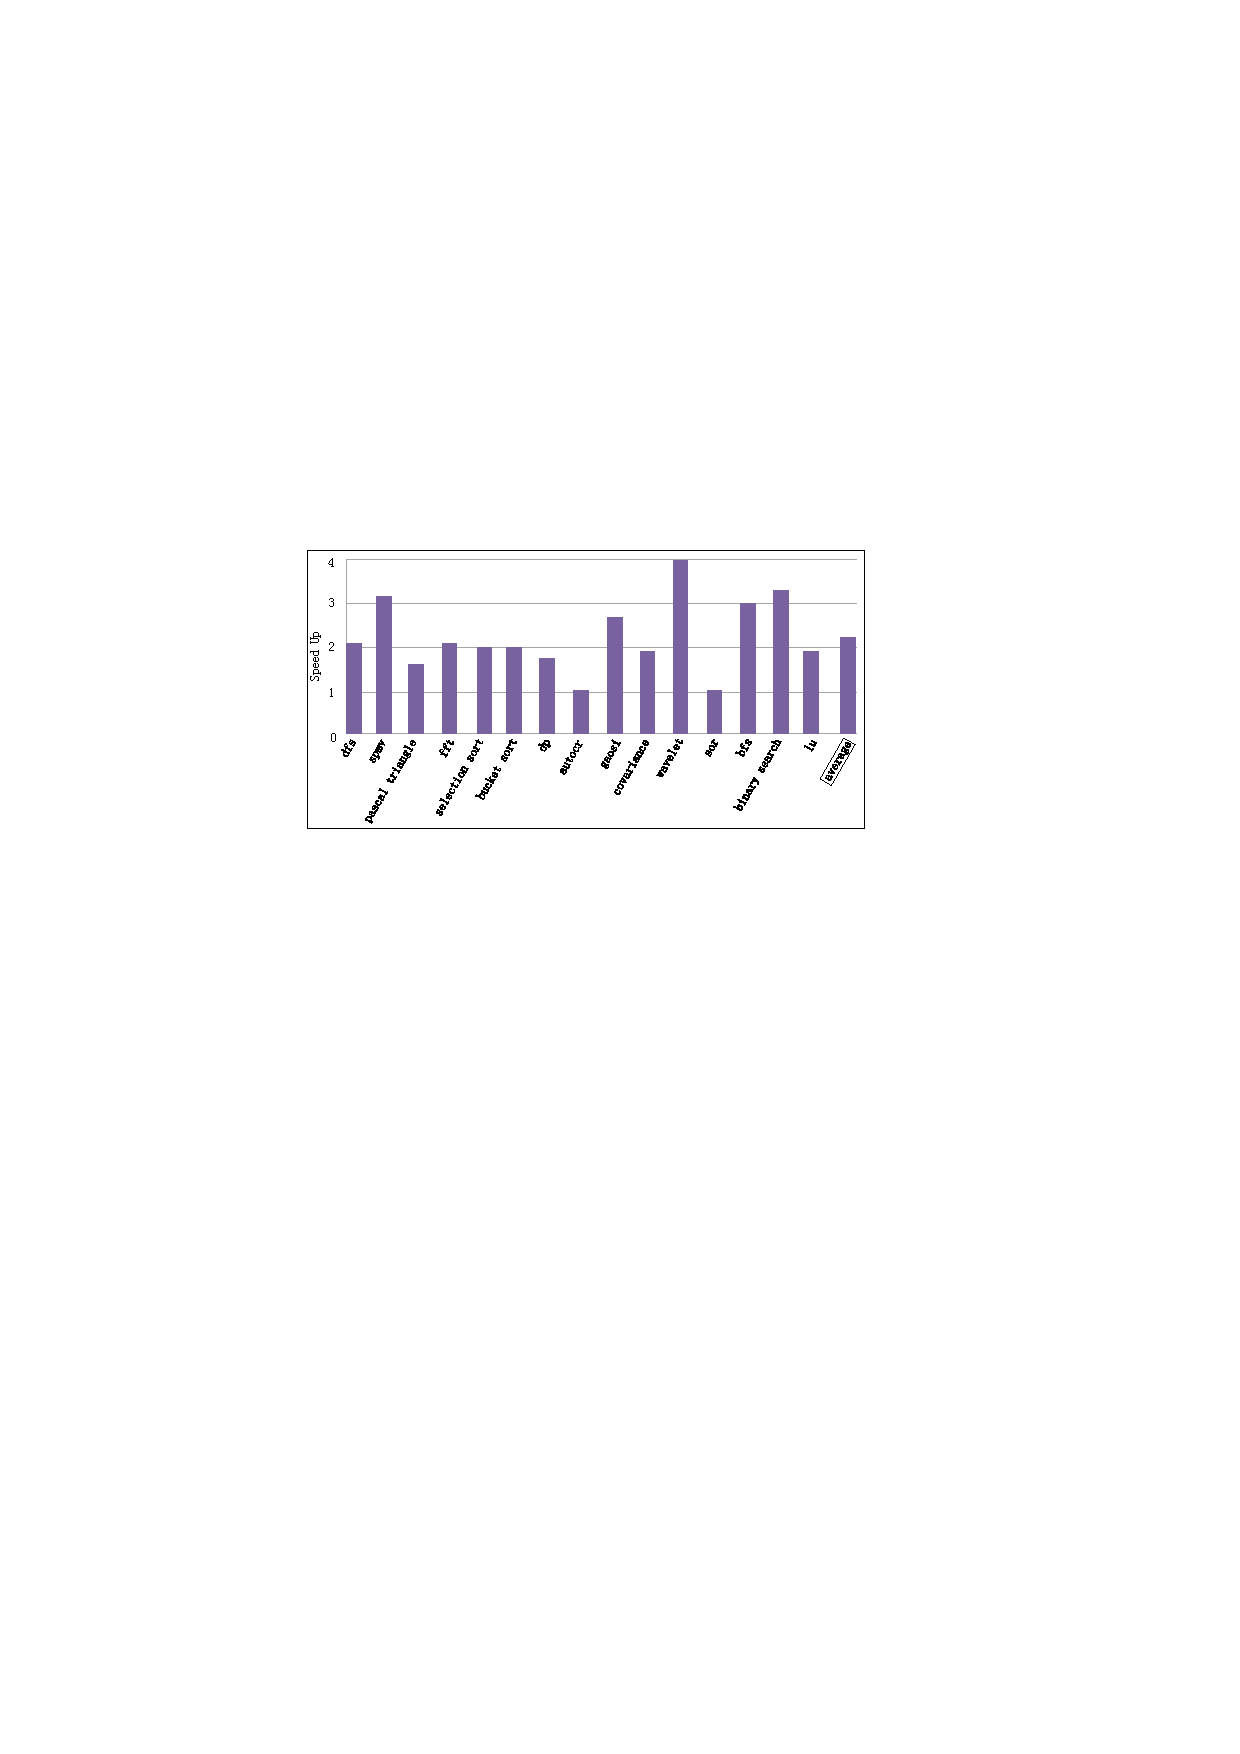
\includegraphics[width=2.5in]{fi/result_1.pdf}%
%\label{fig_first_case}}
%\hfil
%\subfloat[Case II]{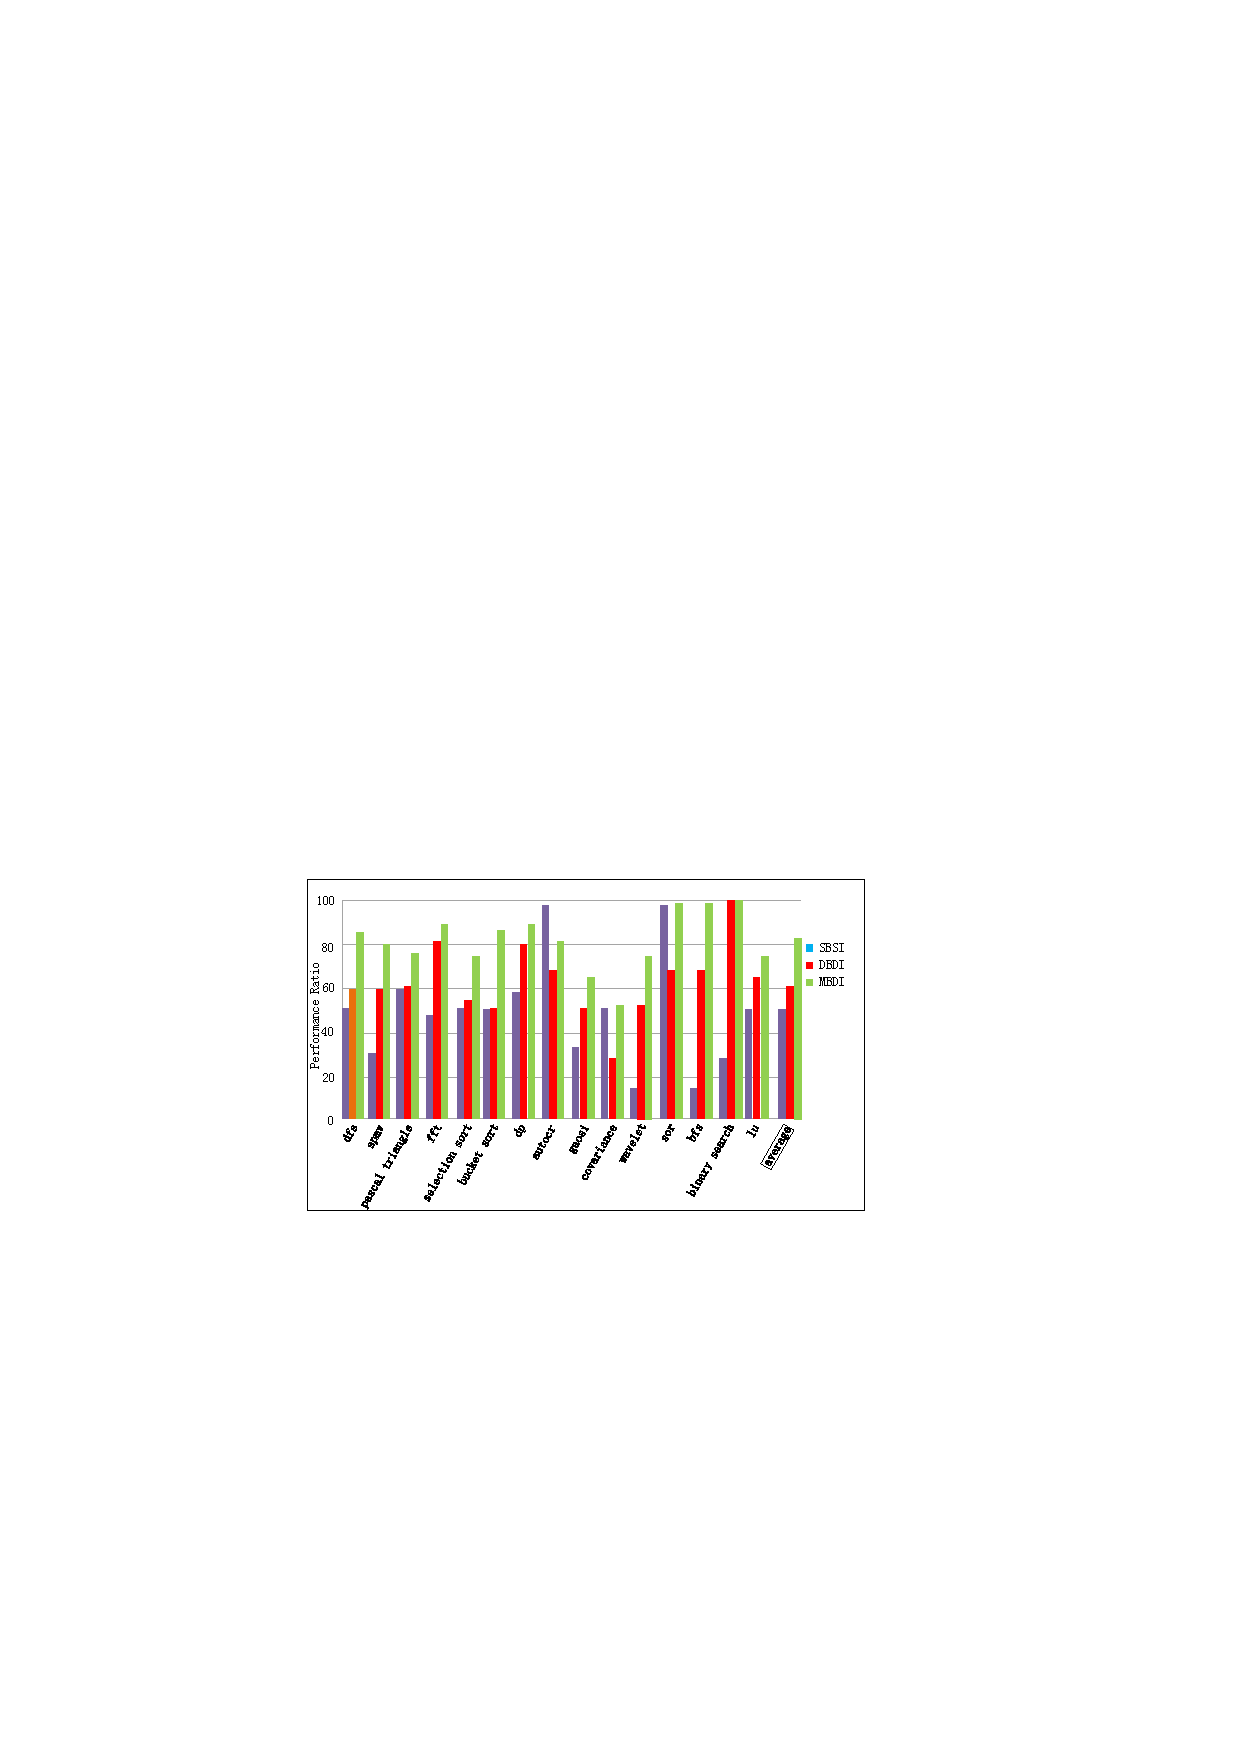
\includegraphics[width=2.5in]{fi/result_2.pdf}%
%\label{fig_second_case}}
%\caption{Simulation results for the network.}
%\label{fig_result}
%\end{figure}

% ???????????2?
%\begin{figure}[ht!]
%	\centering
%	\begin{subfigure}{.4\linewidth}
%		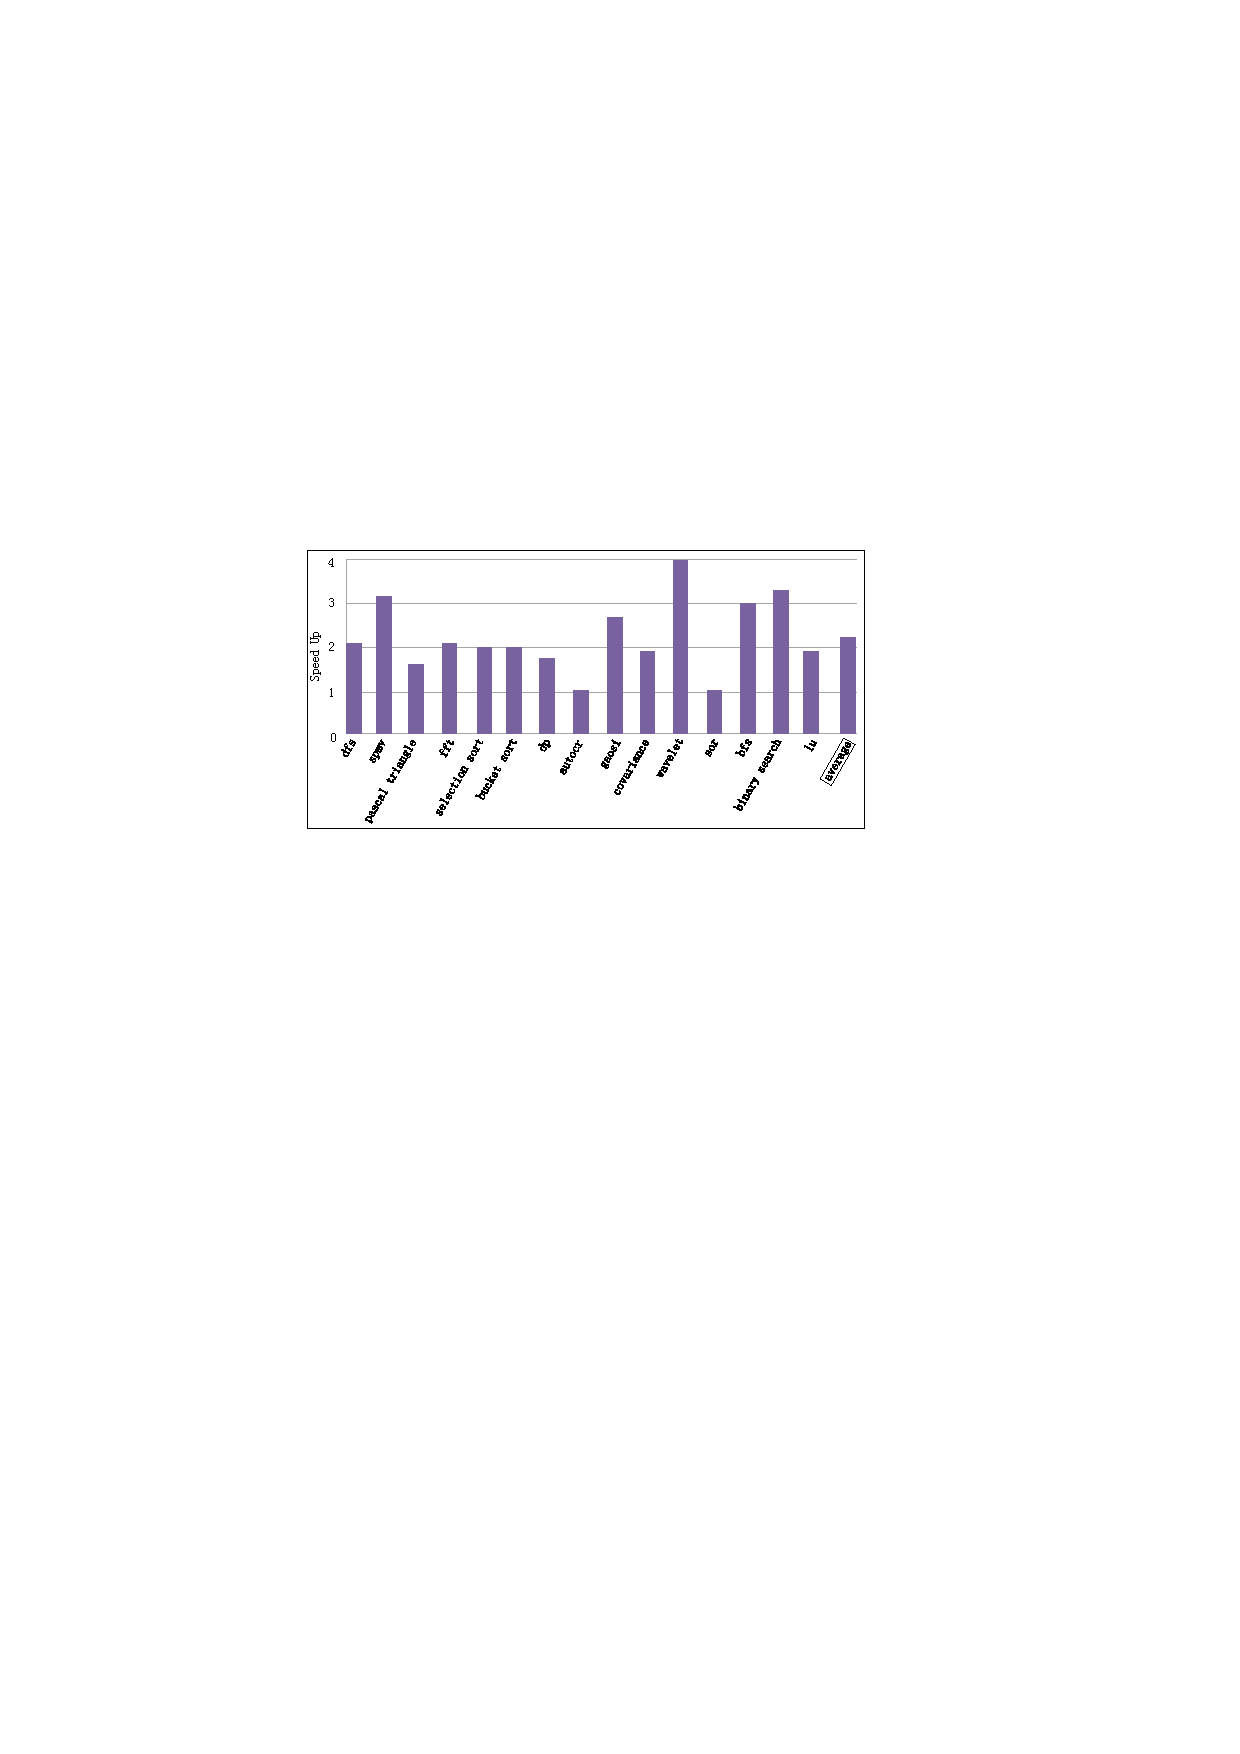
\includegraphics[scale=0.7]{fi/result_1.pdf}
%		\caption{cc}
%	\end{subfigure}
%	\hskip2em
%	\begin{subfigure}{.4\linewidth}
%		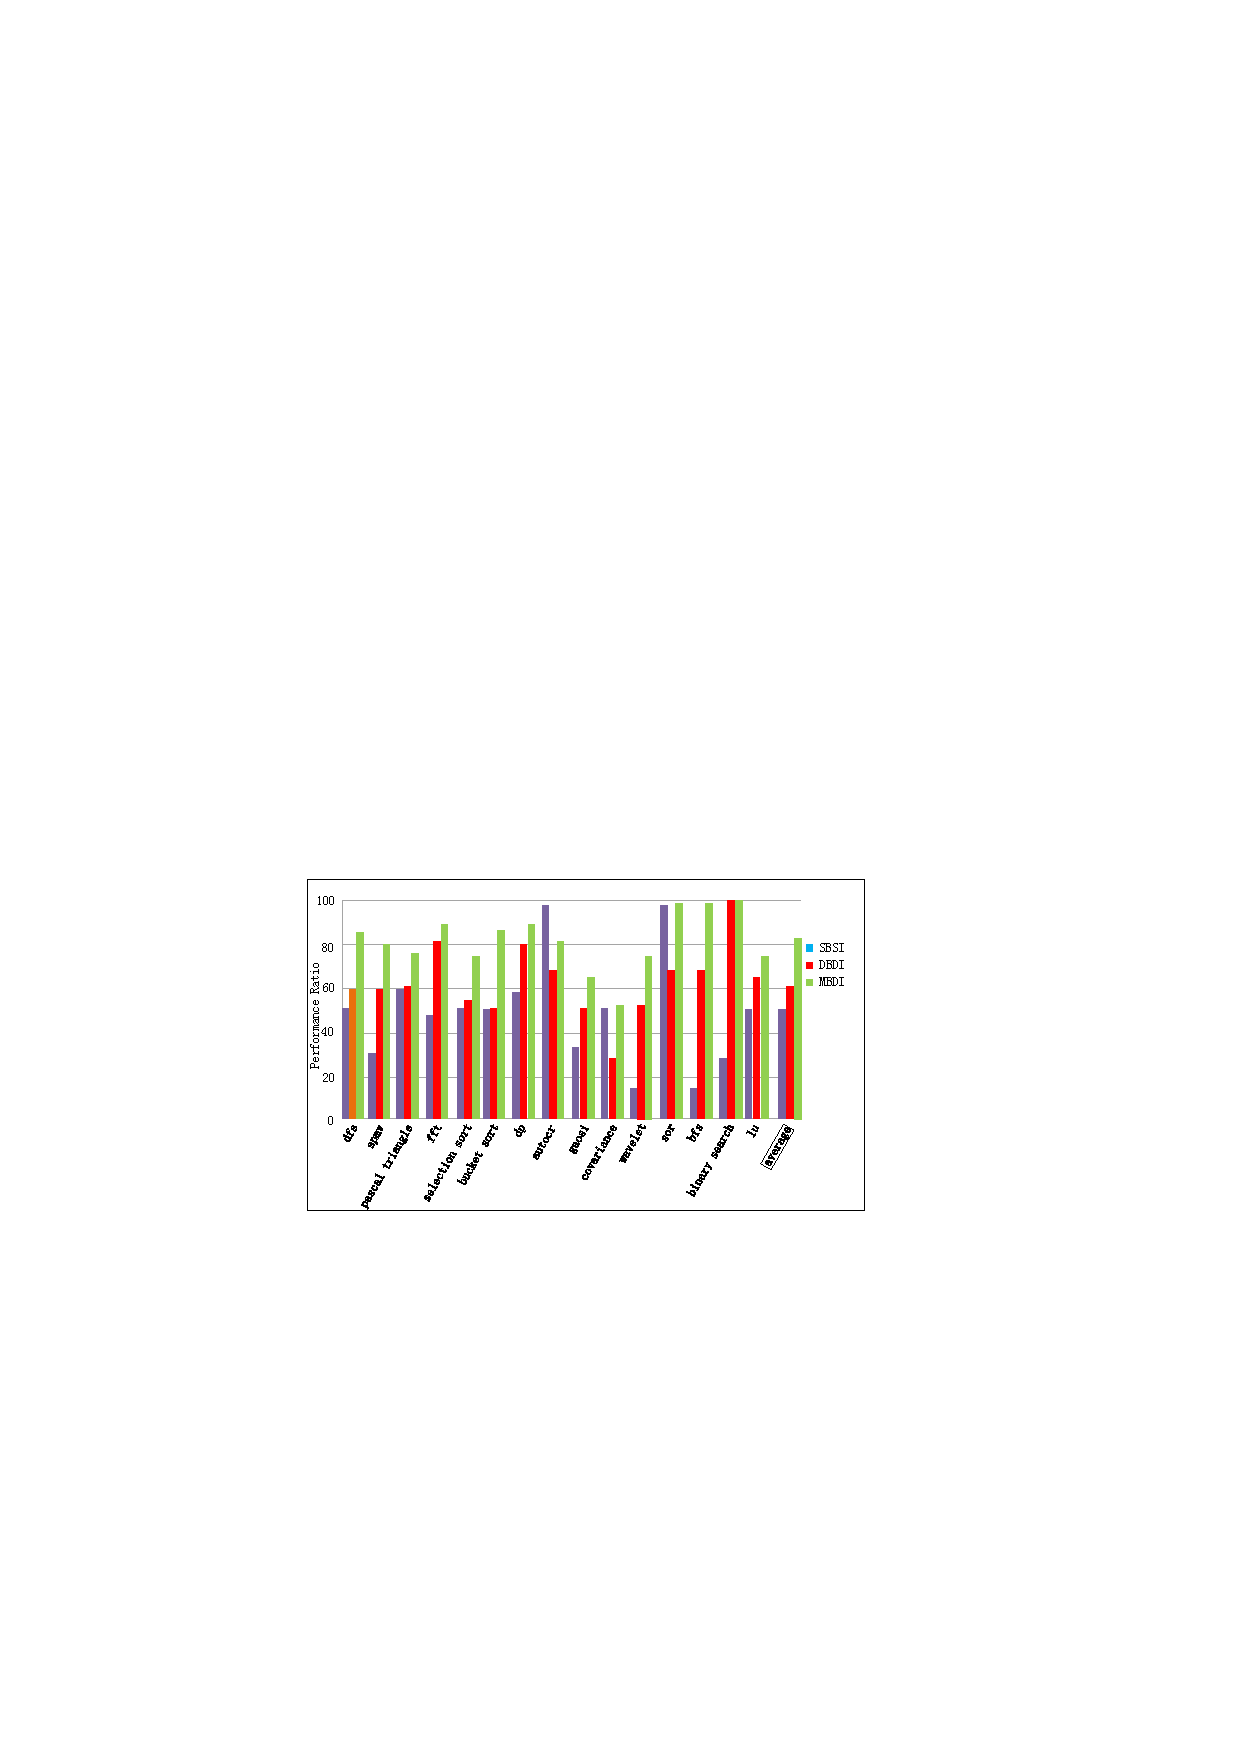
\includegraphics[scale=0.7]{fi/result_2.pdf}
%		\caption{bb}
%	\end{subfigure}
%	\begin{subfigure}{.4\linewidth}
%		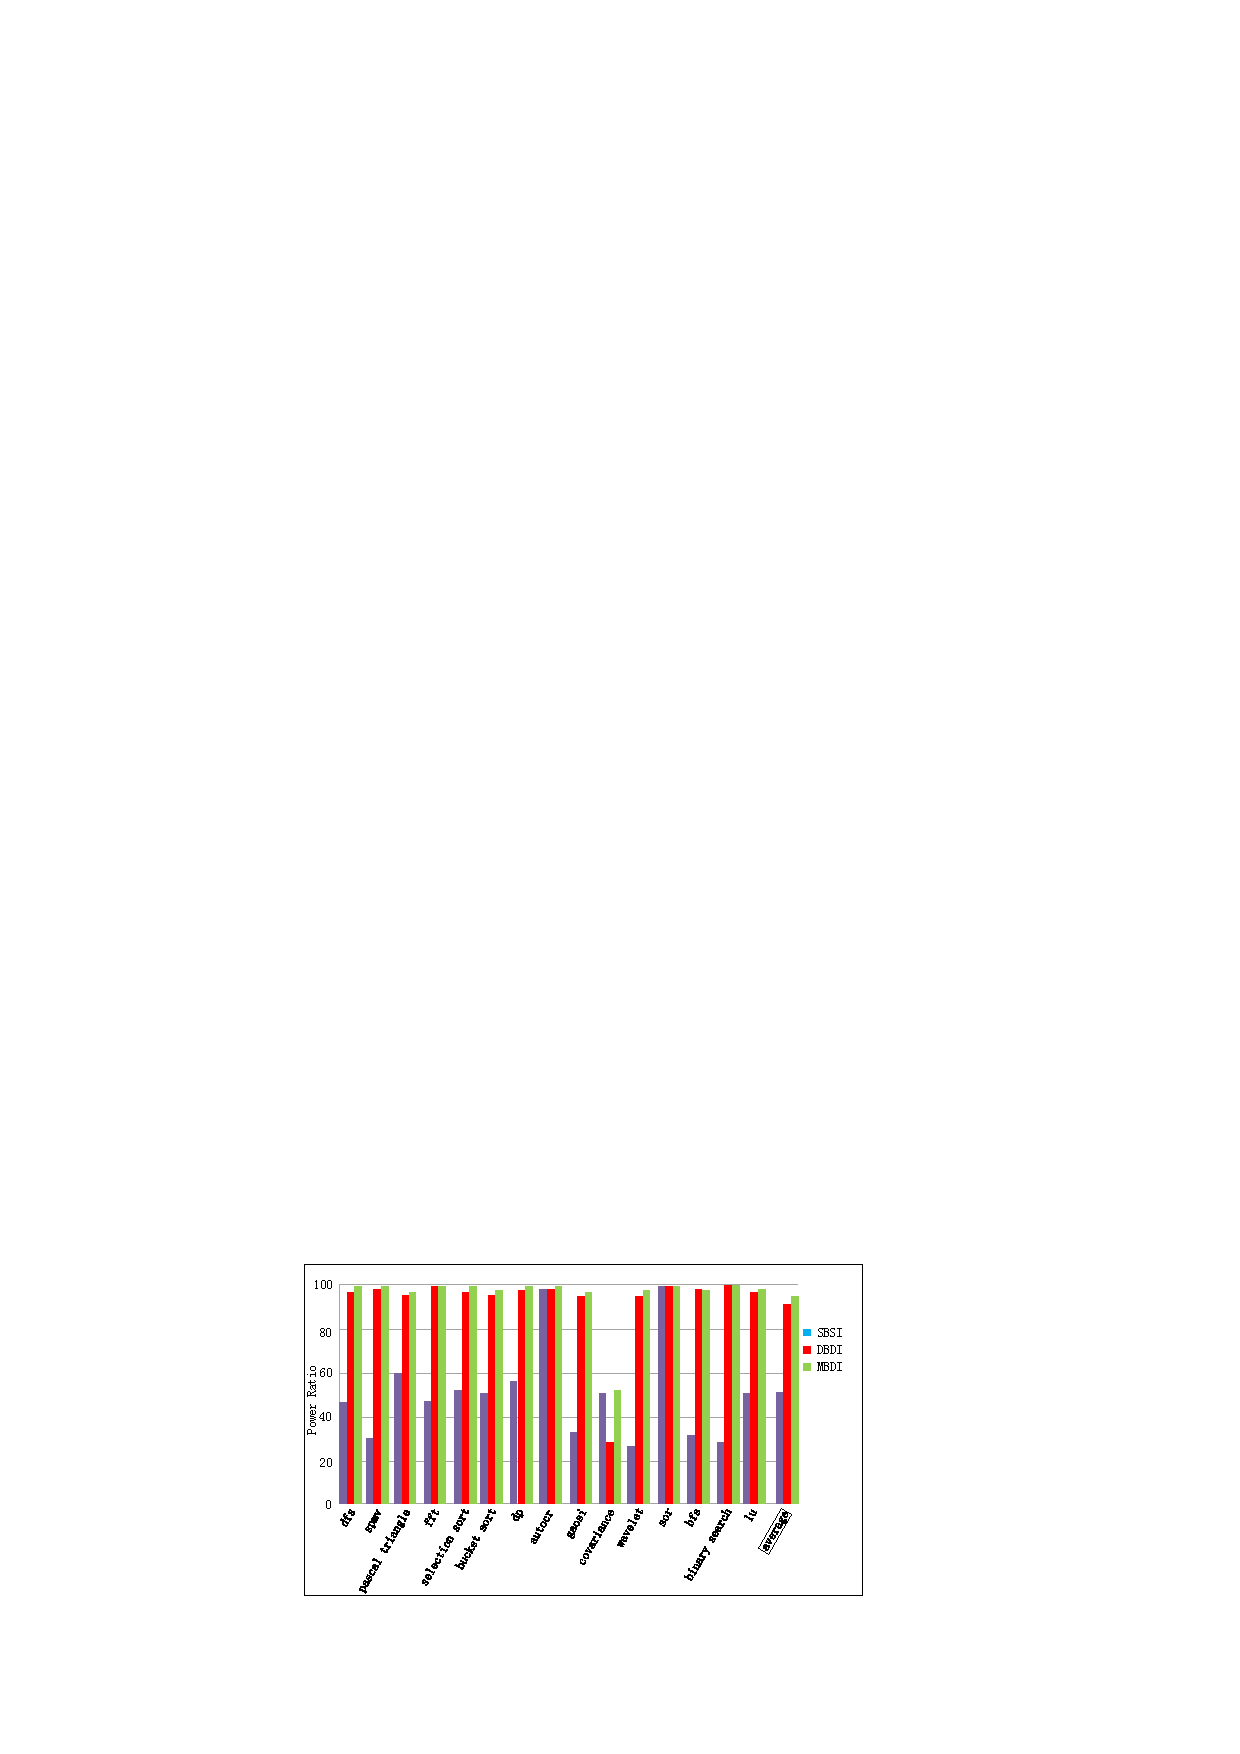
\includegraphics[scale=0.7]{fi/result_3.pdf}
%		\caption{tt}
%	\end{subfigure}
%	\caption{Several subfigures}
%\end{figure}

% https://tex.stackexchange.com/questions/154811/undefined-control-sequence-subfloat
%hen, the code for putting 3 figures side-by-side looks like this:
\begin{figure}[t!]
	\centering
	\begin{subfigure}[b]{0.41\textwidth}
		\centering
		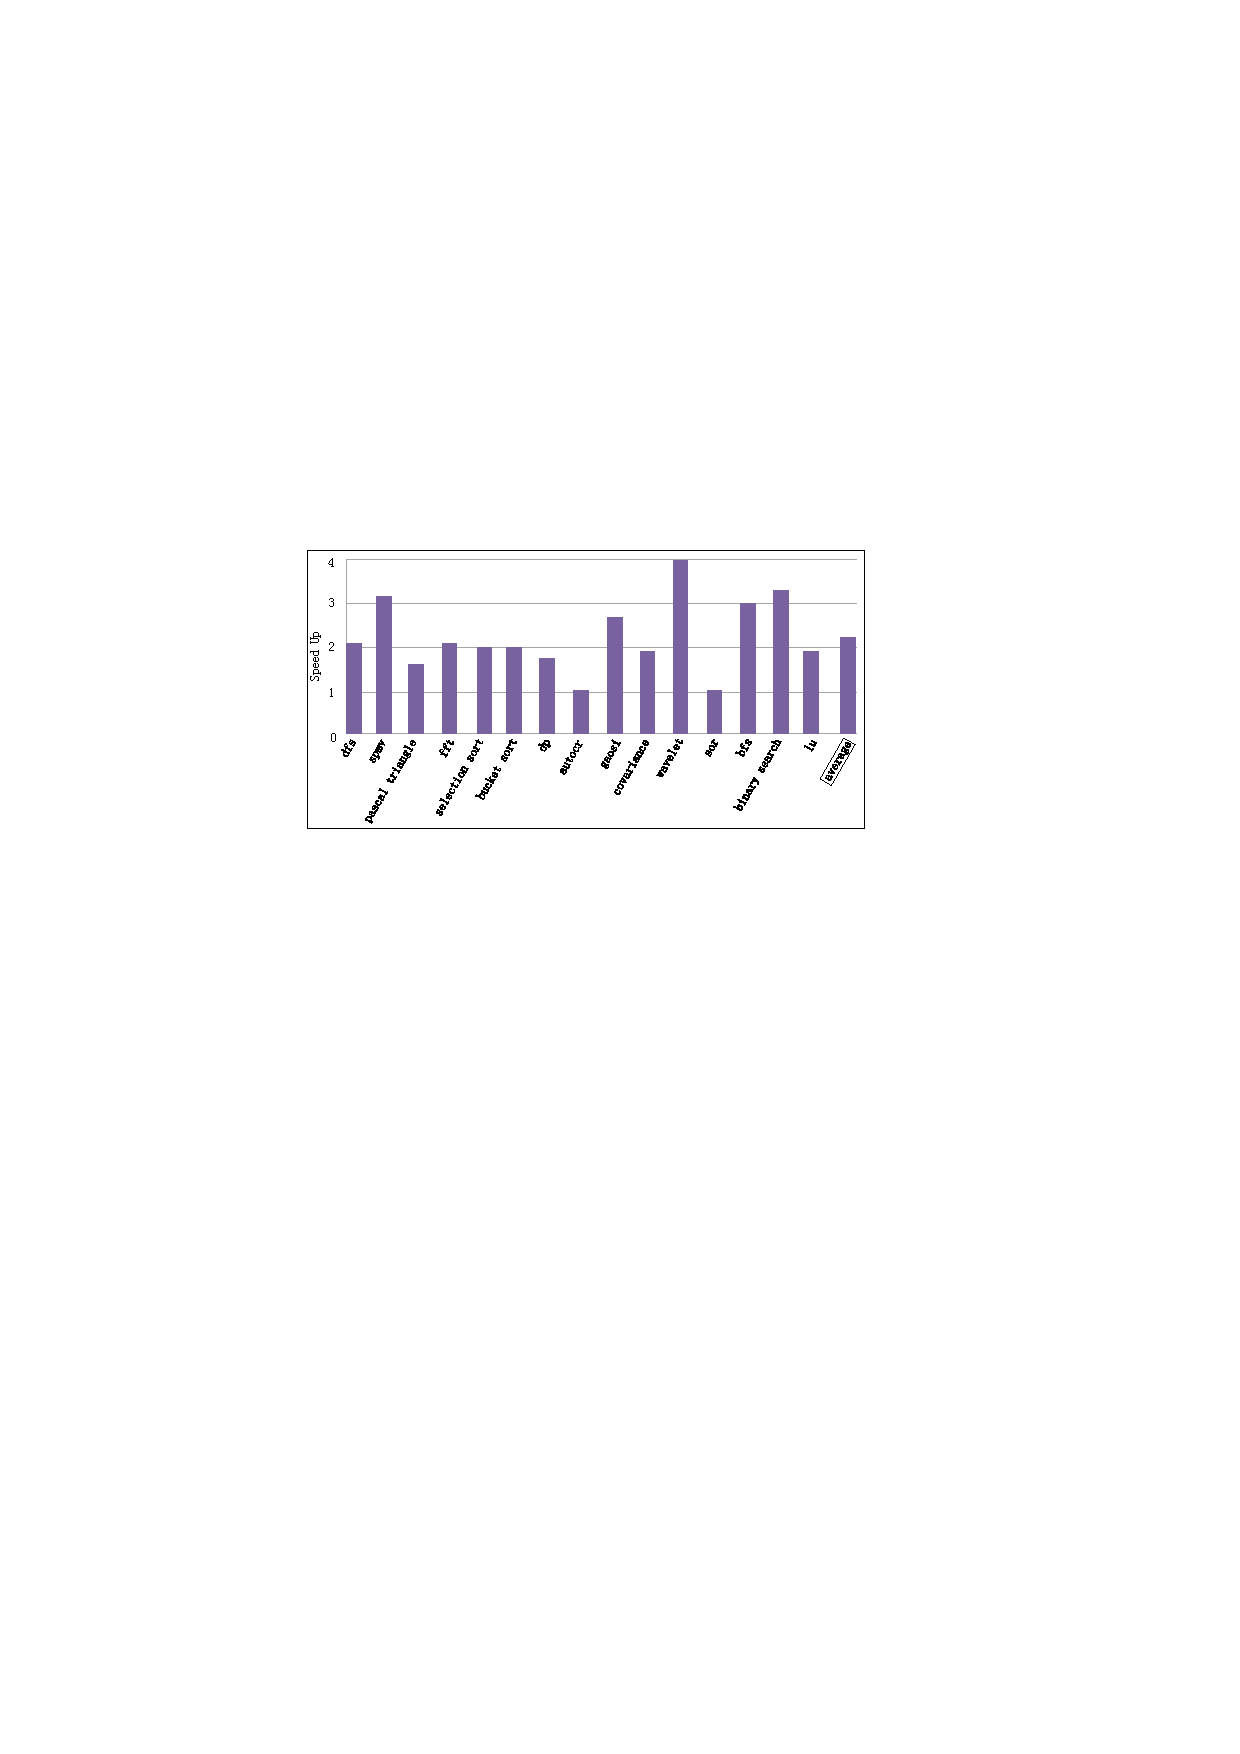
\includegraphics[width=\textwidth]{fi/result_1.pdf}
%		\vspace{-1em}
		\caption{The speed up of DBDI is up to 4x than SBSI based on 15 benchmarks.}
		\label{fig:a}
	\end{subfigure}
	\begin{subfigure}[b]{0.41\textwidth}
		\centering
		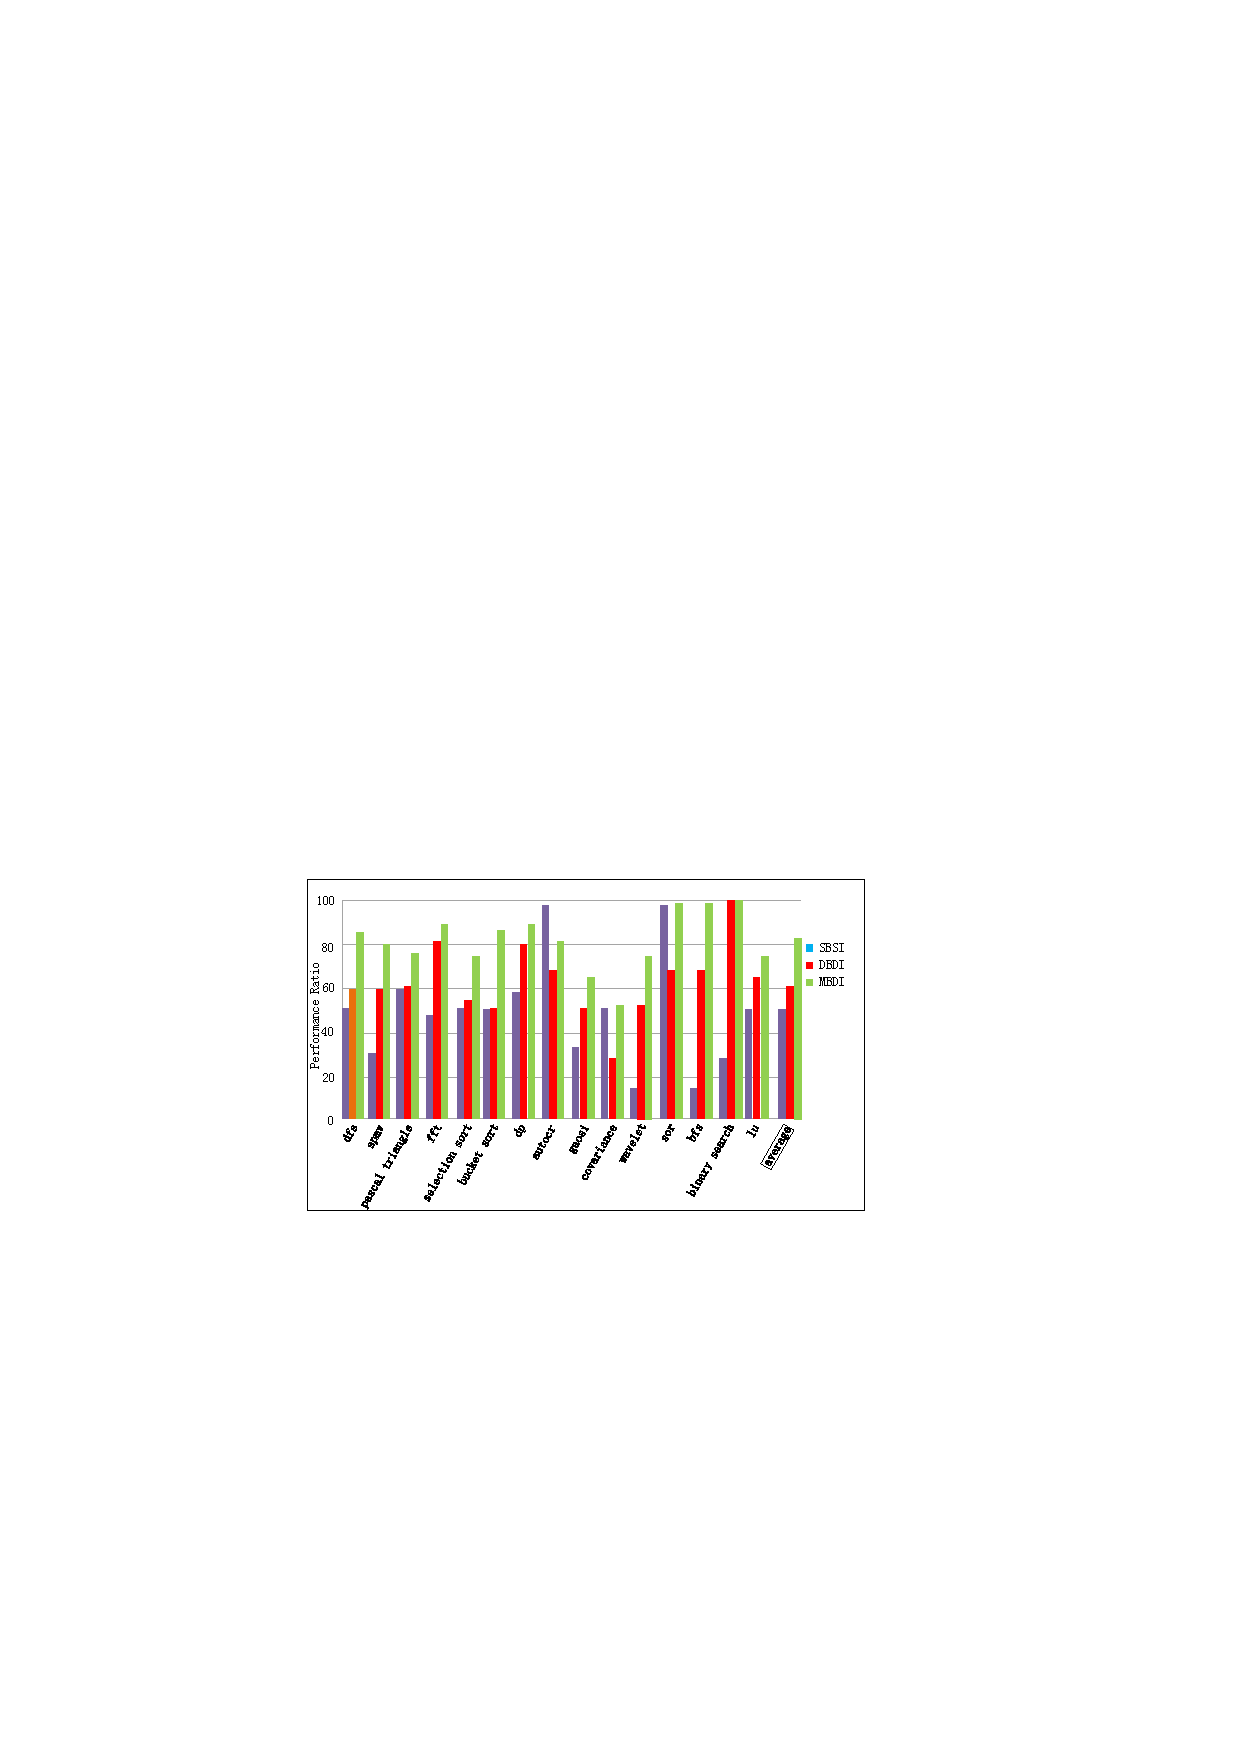
\includegraphics[width=\textwidth]{fi/result_2.pdf}
%		\vspace{-1em}
		\caption{The comparison of performance ratio among SBSI,DBDI and MBDI.}
		\label{fig:b}
	\end{subfigure}
	\begin{subfigure}[b]{0.41\textwidth}
		\centering
		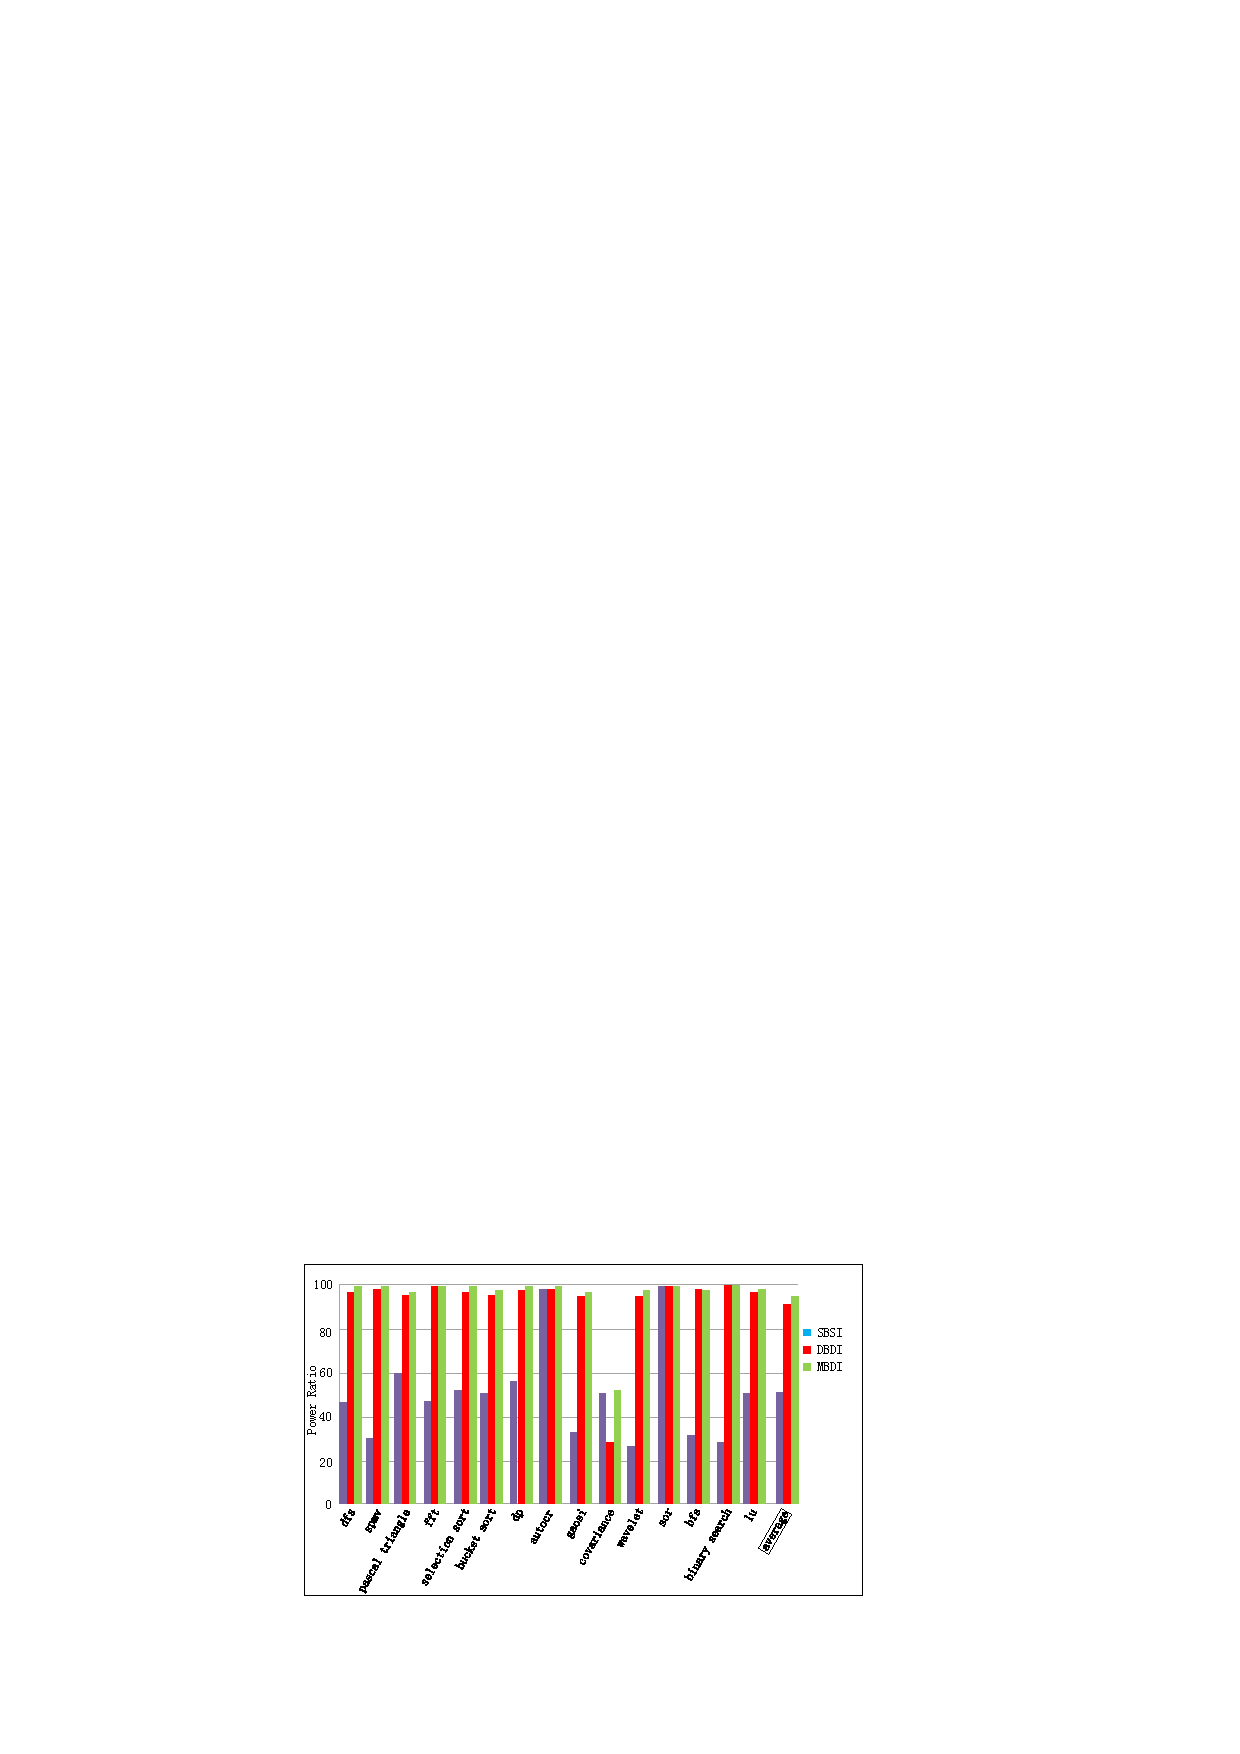
\includegraphics[width=\textwidth]{fi/result_3.pdf}
%		\vspace{-1em}
		\caption{Power efficient is very high for DBDI and MBDI.}
		\label{fig:c}
	\end{subfigure}
%	\vspace{-0.5em}
	\caption{Evaluation for speed, performance and power.}
	\label{fig_result}
\end{figure}

\subsection{Acceleration of DBDI and MBDI}
Alternatively, both $DBDI$ and $MBDI$ are feasible to speed up the program. In Fig. \ref{fig_result}(a), the speed up of 15 applications is larger than 1 as we expected. Specification of speed up is calculated from the time division of $DBDI$ and SBSI. And MBDI has the same effects as $DBDI$. The performance differs greatly in specific application domain. For $wavelet$ and $binary search$ algorithm, the number of dynamic loop layers is larger than others, then $DBDI$ plays an more important role in programs. But the reason why $autocr$ and $sor$ kernel don't achieve commendable performance is that the loop body $m$ is too small. So it is not obvious for the improvement of total performance.

%The different between $DBDI$ and $MBDI$ is that the static loop is as well as operated as dynamic loop. According to the analysis above, the $DBDI$ and $MBDI$ method are efficient as long as there are dynamic loops.
%
%

\subsection{MBDI Improves Efficiency from DBDI}
It is nature that $DBDI$ always achieves a better time performance than SBSI according to Fig. \ref{fig_result}(a) since only a few loops are valid in fact. What's more, the relative performance (in percentage) is described by the division of Minimum Operands and Operands, i.e. $\frac{MO}{O}$. In the same way, specification of relative power is noted by $\frac{MP}{P}$. Therefore, the higher value is much closer to the ideal one.

%
As depicted in Fig. \ref{fig_result}(b), MBDI almost stands for the best situation, only necessary operations are carried out. But $DBDI$ don't perform well in $autocr$,$covariance$ and $sor$, as a matter of fact the loop body $m$ is too small. Thus most of resource are cost in PE0$\sim$PE8 in Fig. \ref{fig_dfg}(e). At the same time, $autocr$,$covariance$ and $sor$ manifest not very well in power as plotted in Fig. \ref{fig_result}(c). The reason why MBDI are always closed to the ideal performance is that it takes only necessary iterations and execute dynamically at crucial time. Sometimes MBDI's performance don't over $90\%$ in Fig. \ref{fig_result}(b), because there are many dynamic loop levels but small innermost loop body. Therefore, the dynamic loop operations are essential and the minimum operands are overidealizing.

It is observed obviously that $DBDI$ and MBDI are always accelerate parallelism program. A principle is also concluded that if the number of inner body is lager than 2($m>2$) for single dynamic loop layer, MBDI are always get the best performance and low power as displayed.
% in  Fig. \ref{fig_result}.


% An example of a floating figure using the graphicx package.
% Note that \label must occur AFTER (or within) \caption.
% For figures, \caption should occur after the \includegraphics.
% Note that IEEEtran v1.7 and later has special internal code that
% is designed to preserve the operation of \label within \caption
% even when the captionsoff option is in effect. However, because
% of issues like this, it may be the safest practice to put all your
% \label just after \caption rather than within \caption{}.
%
% Reminder: the "draftcls" or "draftclsnofoot", not "draft", class
% option should be used if it is desired that the figures are to be
% displayed while in draft mode.
%
%\begin{figure}[!t]
%\centering
%\includegraphics[width=2.5in]{myfigure}
% where an .eps filename suffix will be assumed under latex,
% and a .pdf suffix will be assumed for pdflatex; or what has been declared
% via \DeclareGraphicsExtensions.
%\caption{Simulation Results}
%\label{fig_sim}
%\end{figure}

% Note that IEEE typically puts floats only at the top, even when this
% results in a large percentage of a column being occupied by floats.


% An example of a double column floating figure using two subfigures.
% (The subfig.sty package must be loaded for this to work.)
% The subfigure \label commands are set within each subfloat command, the
% \label for the overall figure must come after \caption.
% \hfil must be used as a separator to get equal spacing.
% The subfigure.sty package works much the same way, except \subfigure is
% used instead of \subfloat.
%
%\begin{figure*}[!t]
%\centerline{\subfloat[Case I]\includegraphics[width=2.5in]{subfigcase1}%
%\label{fig_first_case}}
%\hfil
%\subfloat[Case II]{\includegraphics[width=2.5in]{subfigcase2}%
%\label{fig_second_case}}}
%\caption{Simulation results}
%\label{fig_sim}
%\end{figure*}
%
% Note that often IEEE papers with subfigures do not employ subfigure
% captions (using the optional argument to \subfloat), but instead will
% reference/describe all of them (a), (b), etc., within the main caption.


% An example of a floating table. Note that, for IEEE style tables, the
% \caption command should come BEFORE the table. Table text will default to
% \footnotesize as IEEE normally uses this smaller font for tables.
% The \label must come after \caption as always.
%
%\begin{table}[!t]
%% increase table row spacing, adjust to taste
%\renewcommand{\arraystretch}{1.3}
%% if using array.sty, it might be a good idea to tweak the value of
%% \extrarowheight as needed to properly center the text within the cells
%\caption{An Example of a Table}
%\label{table_example}
%\centering
%% Some packages, such as MDW tools, offer better commands for making tables
%% than the plain LaTeX2e tabular which is used here.
%\begin{tabular}{|c||c|}
%\hline
%One & Two\\
%\hline
%Three & Four\\
%\hline
%\end{tabular}
%\end{table}

%\begin{algorithm}
%	\caption{OMP Algorithm}
%	\begin{algorithmic}[1]
%		\REQUIRE Decomposition of signal $x$
%		\INPUT signal $x \in \mathcal{R}^{m}$, Dictionary $\mathcal{G} \in \mathcal{R}^{m \times n??}$, $\hat{x} = \emptyset$
%		\OUTPUT Decomposed signal $\hat{x}_{\text{est}}$ after $k$ iteration, Residual $R^{(k)}$
%		\STATE \textbf{Initialization} ?$R^{(0)} = x$
%		\WHILE{$i \leq k$}
%		\STATE $l = \displaystyle \argmax_{l = 1,\dots,l} |\langle g_l,R^{(i)} \rangle|$
%		\COMMENT{finding the atom in dictionary $\mathcal{G}$ ?with maximum correlation with residual.}
%		\STATE $R^{(i+1)} = R{(i)}-a_l g_l^{(i)}?$
%		\STATE $\hat{x} = \hat{x}+\langle R^{(i)}, g_{l}^{(i)} \rangle g_{l}^{(i)}?$
%		\STATE $i = i + 1$
%		\ENDWHILE
%	\end{algorithmic}
%\end{algorithm}

% Note that IEEE does not put floats in the very first column - or typically
% anywhere on the first page for that matter. Also, in-text middle ("here")
% positioning is not used. Most IEEE journals/conferences use top floats
% exclusively. Note that, LaTeX2e, unlike IEEE journals/conferences, places
% footnotes above bottom floats. This can be corrected via the \fnbelowfloat
% command of the stfloats package.



\section{Conclusion}
As compiler technologies and advanced mappings skills take important role in CGRA, extracting sophisticated schedule and elegant routing for data communication is feasible. To fill the gap for irregular loop applications, this paper takes loop itself as operations creatively. What's more, a scalability strategy is accommodated to address this challenge. It is verified that the $II$ is only 2 generally but 2x speed up in average. From the experiments, our scheme leads to significant performance improvement and is closed to the desirable one.

% conference papers do not normally have an appendix


% use section* for acknowledgement
%\section*{Acknowledgment}
%This work was supported by the department of Micro/Nano Electronics.

%The authors would like to thank...
%more thanks here


% trigger a \newpage just before the given reference
% number - used to balance the columns on the last page
% adjust value as needed - may need to be readjusted if
% the document is modified later
%\IEEEtriggeratref{8}
% The "triggered" command can be changed if desired:
%\IEEEtriggercmd{\enlargethispage{-5in}}

% references section

% can use a bibliography generated by BibTeX as a .bbl file
% BibTeX documentation can be easily obtained at:
% http://www.ctan.org/tex-archive/biblio/bibtex/contrib/doc/
% The IEEEtran BibTeX style support page is at:
% http://www.michaelshell.org/tex/ieeetran/bibtex/
\bibliographystyle{IEEEtran}
\bibliography{IEEEabrv,ref2}
%\bibliographystyle{IEEEtran}
%% argument is your BibTeX string definitions and bibliography database(s)
%\bibliography{IEEEabrv,ref2}

%
% <OR> manually copy in the resultant .bbl file
% set second argument of \begin to the number of references
% (used to reserve space for the reference number labels box)
%\begin{thebibliography}{1}
%
%\bibitem{IEEEhowto:kopka}
%H.~Kopka and P.~W. Daly, \emph{A Guide to \LaTeX}, 3rd~ed.\hskip 1em plus
%  0.5em minus 0.4em\relax Harlow, England: Addison-Wesley, 1999.
%
%\end{thebibliography}




% that's all folks
\end{document}


